\documentclass[compress]{beamer}
\mode<presentation>
\setbeamercovered{transparent}
\usetheme{Warsaw}
%\useoutertheme{smoothtree}
\usepackage{multirow}
\usepackage[english]{babel}
\usepackage[latin1]{inputenc}
\usepackage{times}
\usepackage[T1]{fontenc}
\usepackage{xmpmulti}
\usepackage{multicol}
\usepackage{colortbl}

%\setbeamersize{text margin left=.25 in,text margin right=.25 in}
\setbeamersize{text margin left=.15 in,text margin right=.15 in}
\usepackage[authoryear]{natbib}


\usepackage{epstopdf}
\usepackage{xcolor}
\usepackage{latexcolors}
%\usepackage[dvipsnames]{xcolor}
\definecolor{antiquebrass}{rgb}{0.8, 0.58, 0.46}
\definecolor{babyblueeyes}{rgb}{0.63, 0.79, 0.95}
\definecolor{babyblue}{rgb}{0.54, 0.81, 0.94}
\definecolor{bistre}{rgb}{0.24, 0.17, 0.12}
\definecolor{brightlavender}{rgb}{0.75, 0.58, 0.89}
\definecolor{bulgarianrose}{rgb}{0.28, 0.02, 0.03}
\definecolor{slateblue}{rgb}{0.56, 0.74, 0.56}
\definecolor{cordovan}{rgb}{0.54, 0.25, 0.27}
\definecolor{darkbyzantium}{rgb}{0.36, 0.22, 0.33}

\setbeamercolor{structure}{fg=airforceblue!80, bg= black!60}







\usepackage{tikz}
\usetikzlibrary{shadows,calc}
\usetikzlibrary{shadows.blur}
\usetikzlibrary{shapes.symbols}
\usepackage{hyperref}
\usepackage{booktabs}
\usepackage{colortbl}
\usepackage{multirow}
%%%%%%%%% shaddow image %%%%%
% some parameters for customization
\def\shadowshift{3pt,-3pt}
\def\shadowradius{6pt}
\colorlet{innercolor}{black!60}
\colorlet{outercolor}{gray!05}
% this draws a shadow under a rectangle node
\newcommand\drawshadow[1]{
\begin{pgfonlayer}{shadow}
    \shade[outercolor,inner color=innercolor,outer color=outercolor] ($(#1.south west)+(\shadowshift)+(\shadowradius/2,\shadowradius/2)$) circle (\shadowradius);
    \shade[outercolor,inner color=innercolor,outer color=outercolor] ($(#1.north west)+(\shadowshift)+(\shadowradius/2,-\shadowradius/2)$) circle (\shadowradius);
    \shade[outercolor,inner color=innercolor,outer color=outercolor] ($(#1.south east)+(\shadowshift)+(-\shadowradius/2,\shadowradius/2)$) circle (\shadowradius);
    \shade[outercolor,inner color=innercolor,outer color=outercolor] ($(#1.north east)+(\shadowshift)+(-\shadowradius/2,-\shadowradius/2)$) circle (\shadowradius);
    \shade[top color=innercolor,bottom color=outercolor] ($(#1.south west)+(\shadowshift)+(\shadowradius/2,-\shadowradius/2)$) rectangle ($(#1.south east)+(\shadowshift)+(-\shadowradius/2,\shadowradius/2)$);
    \shade[left color=innercolor,right color=outercolor] ($(#1.south east)+(\shadowshift)+(-\shadowradius/2,\shadowradius/2)$) rectangle ($(#1.north east)+(\shadowshift)+(\shadowradius/2,-\shadowradius/2)$);
    \shade[bottom color=innercolor,top color=outercolor] ($(#1.north west)+(\shadowshift)+(\shadowradius/2,-\shadowradius/2)$) rectangle ($(#1.north east)+(\shadowshift)+(-\shadowradius/2,\shadowradius/2)$);
    \shade[outercolor,right color=innercolor,left color=outercolor] ($(#1.south west)+(\shadowshift)+(-\shadowradius/2,\shadowradius/2)$) rectangle ($(#1.north west)+(\shadowshift)+(\shadowradius/2,-\shadowradius/2)$);
    \shade[outercolor,right color=innercolor,left color=innercolor] ($(#1.north west)+(-\shadowradius/12,\shadowradius/12)$) rectangle ($(#1.south east)+(\shadowradius/12,-\shadowradius/12)$);%Frame
    \filldraw ($(#1.south west)+(\shadowshift)+(\shadowradius/2,\shadowradius/2)$) rectangle ($(#1.north east)+(\shadowshift)-(\shadowradius/2,\shadowradius/2)$);
\end{pgfonlayer}
}
% create a shadow layer, so that we don't need to worry about overdrawing other things
\pgfdeclarelayer{shadow} 
\pgfsetlayers{shadow,main}
% Define image shadow command
\newcommand\shadowimage[2][]{%
\begin{tikzpicture}
\node[anchor=south west,inner sep=0] (image) at (0,0) {\includegraphics[#1]{#2}};
\drawshadow{image}
\end{tikzpicture}}
\usepackage{calligra}

\DeclareMathOperator*{\argmax}{Arg\,max}
\DeclareMathOperator*{\argmin}{Arg\,min}
\newcommand{\norm}[1]{\left\Vert #1 \right\Vert }
\newcommand{\bbetaHat}{ \widehat{\bbeta}}
\newcommand{\bbetaLSE}{ \widehat{\bbeta}_{_{\text{LSE}}}}
\newcommand{\bbetaMLE}{ \widehat{\bbeta}_{_{\text{MLE}}}}
\newcommand{\sqBullet}[1]{  {\tiny \tiny \tiny \qBoxCol{#1!60}{ }} }
%***************
%\newtheorem{thm}{Theorem}
%\documentclass[noinfoline]{imsart}
%\usepackage{amsmath,amstext,amssymb}
%%\usepackage[top=1.5in, bottom=1.5in, left=1.2in, right=1.2in]{geometry}
%% settings
%%\pubyear{2005}
%%\volume{0}
%%\issue{0}
%%\firstpage{1}
%%\lastpage{8}
%\arxiv{arXiv:0000.0000}

%\startlocaldefs
%\numberwithin{equation}{section}
%\theoremstyle{plain}
%\newtheorem{thm}{Theorem}
%\endlocaldefs
\usepackage{lipsum} 
\usepackage{amsmath}
\usepackage{amssymb}
\usepackage{amsbsy} 
\usepackage{amsthm}
\usepackage{mathrsfs}
\usepackage{eufrak}
\usepackage{mathrsfs}
\usepackage{color}
\usepackage{verbatim}
\usepackage{graphicx}
\usepackage{bm}
\usepackage{enumerate}
\usepackage{epstopdf} 
\usepackage{natbib}
\usepackage{undertilde}
%\RequirePackage[colorlinks,citecolor=blue,urlcolor=blue]{hyperref}
%\usepackage{subfig}
\usepackage[final]{pdfpages}

\usepackage{algorithm}  %@subhajit
\usepackage{algpseudocode} %@subhajit
\usepackage{algorithmicx}     %@subhajit
\usepackage{undertilde}


\newcommand{\sphere}{{\mathbb{S}}}
\newcommand{\R}{\mathbb{R}}
\newcommand{\LatentV}{V}
\newcommand{\NC}{m}
\newcommand{\Priorf}{f_{prior}}
\newcommand{\FWOne}[2]{{{}_{1}\Psi _{1}\left[{\begin{matrix}(\frac{#1}{2},\frac{1}{2})\\(1,0)\end{matrix}};#2\right]} 
}


\newcommand{\HyPriorMu}{\thetabf}
\newcommand{\HyPriorAlpha}{\alpha}
\newcommand{\HyPriorBeta}{\beta}
\newcommand{\HyPriorK}{\zeta}
\newcommand{\Indicator}[2]{\mathbb{I}_{_{#1}}({#2 })}
\newcommand{\xb}{\bm{x}}
\newcommand{\bx}{\MakeVec{\bm{x}}}
\newcommand{\bX}{\bm{X}}
\newcommand{\by}{\MakeVec{\bm{y}}}
\newcommand{\bZ}{\bm{Z}}
\newcommand{\bF}{\bm{F}}
\newcommand{\btheta}{\MakeVec{{\bm{\theta}}}}
\newcommand{\Bpi}{\MakeVec{\boldsymbol{\pi}}}
\newcommand{\thetabf}{\MakeVec{\boldsymbol{\theta}}}
\newcommand{\Thetabf}{\boldsymbol{\Theta}}
\newcommand{\taubf}{\MakeVec{\boldsymbol{\tau}}}
\newcommand{\Tr}{Tr}


\newcommand{\bM}{\bm{M}}
\newcommand{\bD}{\MakeVec{\bm{D}}}
\newcommand{\bV}{\MakeVec{\bm{V}}}
\newcommand{\loglikmix}{\mathcal{L}_{\bM,\bD,\bV}}
\newcommand{\hypdc}{{}_0F_1\left(\frac{n}{2},\frac{D_c^2}{4}\right)}


\usepackage{xstring}
\usepackage[normalem]{ulem}
\definecolor{ultramarine}{RGB}{38,29,163}
\newcommand\PalDel[1]{{\color{red} {\sout{#1}}}}
\newcommand\Pal[1]{{\color{ultramarine}{#1}}}
\newcommand\PalRp[2]{\PalDel{#1} \Pal{#2}}
\newcommand\PalCmnt[1]{{\color{ultramarine} {[[[***PAL:  #1 ***]]]}}}

\newcommand{\qedwhite}{\hfill \ensuremath{\Box}}
\newcommand{\SpaceD}{\mathcal{S}_p}
\newcommand{\SpaceM}{\widetilde{\mathcal{V}}_{n,p}}
\newcommand{\SpaceV}{\mathcal{V}_{p,p}}
\newcommand{\SpaceF}{\mathbb{R}^{n,p}}
\newcommand{\StiefelS}{\mathcal{V}_{n,p}}
\newcommand{\SpacePi}{\mathbb{S}_{\pi}}
\newcommand{\ML}{{\cal{ML}}}
\newcommand{\ProdSpace}{\boldsymbol{\Theta}}
\newcommand{\ThetaAndPi}{\Xi}
\newcommand{\ClassML}{\mathcal{C}_{\ML}}


\newcommand{\balpha}{\MakeVec{\bm{\alpha}}}
\newcommand{\bbeta}{\MakeVec{\bm{\beta}}}
\newcommand{\bEta}{\bm{\eta}}
\newcommand{\bd}{{\utilde{\bm{d}}}}
\newcommand{\BoEta}{{\utilde{\boldsymbol{\eta}}}}
%\newtheorem{theorem}{Theorem}[section]
%\newtheorem{theorem}{Theorem}
%\newtheorem{lemma}{Lemma}
%\newtheorem{result}{Result}
\newtheorem{defn}{Definition}
\newcommand{\pdv}[2][]{\frac{\partial#1}{\partial#2}}
\newcommand{\pdvtwo}[2][]{\frac{\partial^2#1}{{\partial#2}^2}}


%\newcommand{\mubf}{\boldsymbol{\mu}}
\newcommand{\mubf}{\MakeVec{\mu}}
\newcommand{\sumI}{ \sum_{i=1}^{n}}
\newcommand{\Ybar}{{\overline{Y}}}

\newcommand{\Expectation}[1]{\mathbb{E}{[#1]}}
\newcommand{\priorXzero}{\Psi}
\newcommand{\iMat}{\mathbf{I}_{p}}

% 
% \newtheorem{thm}{Theorem}[section]
% \newtheorem{cor}[thm]{Corollary}
% \newtheorem{lem}[thm]{Lemma}
%\newtheorem{proposition}{Proposition}

%\newtheorem{theorem}{Theorem}[chapter]%To link the theorem to each chapter uncomment the chapter option
%\newtheorem{lemma}{Lemma}%[theorem]% To link each lemma to a theorem uncomment the theorem option
%\newtheorem{corollary}{Corollary}%[theorem]% To link each corollary to a theorem uncomment the theorem option
% to link a corollary to a chapter change the theorem option to chapter
%\newtheorem{definition}{Definition}%[chapter] %the same is true for both definitions and assumptions
\newtheorem{assumption}{Assumption}%[chapter] %
%\newtheorem{proposition}{Proposition}[chapter]
%\newtheorem{fact}{Fact} %%% added by @subho
\newcommand{\StrongNBD}[2]{S_{#1}{#2}}
\newcommand{\bpi} {\boldsymbol{\pi}}
\newcommand{\bphi} {\boldsymbol{\phi}}
\newcommand{\bb}[1]{\boldsymbol{#1}}
% Definitions of handy macros can go here

\newcommand{\normtwo}[1]{{\left\lVert#1\right\rVert}_2}

\newcommand{\dataset}{{\cal D}}
\newcommand{\fracpartial}[2]{\frac{\partial #1}{\partial  #2}}
\newcommand{\Lesbegue}[1]{\mu_{\btheta_{#1},\bpi_{#1}}}
\newcommand{\fthetapi}[1]{f_{\btheta_{#1},\bpi_{#1}}}
% Heading arguments are {volume}{year}{pages}{submitted}{published}{author-full-names}
\newcommand{\doublehat}[1]{%
    \settoheight{\dhatheight}{\ensuremath{\widehat{#1}}}%
    \addtolength{\dhatheight}{-0.35ex}%
    \widehat{\vphantom{\rule{2pt}{\dhatheight}}%
    \smash{\hspace{-0.5mm}\widehat{#1}}}}

\newcommand{\hyp}{{}_0F_1\left(\frac{n}{2},\frac{D^2}{4}\right)}
\newcommand{\hypinline}{{}_0F_1\left({n}/{2},{D^2}/{4}\right)}

\newcommand{\partialhyp}[1]{\frac{\partial}{\partial\,{d_{#1}}}\,\left[\hyp\right]}

\newcommand{\fracProbZ}[1]{\frac{\langle Z_{ic} \rangle \, #1}{\sum_{i=1}^{N} \langle Z_{ic}\rangle  } }
\newcommand{\EmVar}[1]{\widetilde{#1}^{(c)}}

\newcommand{\IMDY}{{\it{CCPD}}}
\newcommand{\JMDY}{{\it{JCPD}}}

\newcommand{\DYlang}{\frac{\exp(\nu\,\bEta^T\bd)}{{\left[{}_0F_1\left(\frac{n}{2},\frac{D^2}{4}\right)\right]}^{\nu}}}

\newcommand{\logDYlang}{\nu\,\bEta^T\bd - \nu\,\log\left({}_0F_1\left(\frac{n}{2},\frac{D^2}{4}\right)\right)}

\newcommand{\lhyp}{\log\left({}_0F_1\left(\frac{n}{2},\frac{D^2}{4}\right)\right)}

%\jmlrheading{1}{2000}{1-48}{4/00}{10/00}{SS \& JH \& AB}

% Short headings should be running head and authors last names

%\ShortHeadings{BDP and cIBP}{SS \& JH \& AB}
%\firstpageno{1}

\newcommand{\diam}[1]{{{#1}^{\ast}}}

%%% coloring option %%%
\definecolor{auburn}{rgb}{0.53, 0.1, 0.5}
\newcommand{\sss}{\color{auburn}}  %%% for Subhajit
\newcommand{\sse}{\color{black}}
\newcommand{\attn}{\color{red}}
\newcommand{\rms}{\color{magenta}}  %%% for Riten
\newcommand{\rme}{\color{black}}
\newcommand{\MLDensity}{f_{\ML}}
\setlength{\parindent}{0cm}
\newcommand{\posterior}

\newcommand{\variableX}{\bd}
\newcommand{\funch}{\mathfrak{h}}
\newcommand{\IndVzero}[1]{\mathbb{I}({X\in \mathcal{V}^{#1}_0})}
\newcommand{\Rnp}{\mathbb{R}^{n \times p}}
\newcommand{\Rpp}{\mathbb{R}^{p \times p}}
\newcommand{\vecnorm}[1]{\lVert #1\rVert}

\newcommand{\etapsiD}{\eta_{\priorXzero}}
\newcommand{\BoEtapsiD}{\BoEta_{\priorXzero}}

\newcommand{\DMp}{\mathcal{D}^{p \times p}}
\newcommand{\Rplus}{\mathbb{R}_{+}}
\newcommand{\prodMeasure}{\Upsilon}

\newcommand{\m}{{\bf m_{\BoEta}}} 
\newcommand{\SetWithMode}{\mathcal{S}}
\newcommand{\SetWithModePrime}{\mathcal{S}}
\newcommand{\TargetComp}{\mathcal{S}^{\star}}

\newcommand{\ConstCondDen}{K_{\nu, \BoEta}} 

\newcommand{\hyparam}[2]{
    \IfEqCase{#1}{
        {M}{\xi^{#2}_c}
        {V}{\gamma^{#2}_c}%
        
    }
  }
\newcommand{\threepartdef}[6]
{
	\left\{
		\begin{array}{lll}
			#1 & \mbox{if } #2 \\
			#3 & \mbox{if } #4 \\
			#5 & \mbox{if } #6
		\end{array}
	\right.
}

\def\bv{\color{blue}}
\def\ev{\color{black}}
\newcommand{\bch}{\bv }
\newcommand{\ech}{\ev\normalsize}
%\newcommand{\MakeVec}[1]{{\utilde{\bf #1}}}
\newcommand \Measure[2][]{%
  \ifstrempty{#1}{
  \IfEqCase{#2}{
        {M}{\mu}%
        {D}{\mu_1}%
        {V}{\mu_2}
        {X}{\mu}
   }  
  }{
  \IfEqCase{#1}{
  {1}{
   \IfEqCase{#2}{
        {M}{d\mu(M)}%
        {D}{d\mu_1(\bd)}%
        {V}{d\mu_2(V)}
        {X}{d\mu(X)}
        {Y}{d\mu(Y)}
        {MDV} {d\mu(M)\; d\mu_1(\bd) \;d\mu_2(V) }
        }
   } 
   {2}{
   \IfEqCase{#2}{
         {M}{d\mu(M^{\ast})}%
        {D}{d\mu_1(\bd^{\ast})}%
        {V}{d\mu_2(V^{\ast})}
        {X}{d\mu(X^{\ast})}
        }
   }
   {3}{
   \IfEqCase{#2}{
         {M}{\mu(dM^{\star})}%
        {D}{\mu_2(d\bd^{\star})}%
        {V}{\mu_1(dV^{\star})}
        {X}{\mu(X^{\star})}
        }
   }   
   
   } 
  }%
}
  \newcommand{\VONF}{\text{VonMisesFisher}}
\newcommand{\MPGalpha}{\alpha}
\newcommand{\MPGnu}{\nu}
\newcommand{\MPG}{MPG }
\newcommand{\ybin}{y^{(\text{bin})}}


%\newcommand{\abs}[1]{\left \vert  #1  \right\vert  }
\usepackage{caption}
\usepackage{subcaption}

%%%%%%%%%%%%%%%%%%%%%%%%%%%
\newcommand{\IEHC}{\text{IEHC}}







\newcommand \Th[1]{%
  \IfEqCase{#1}{
        {1}{ 1^{\text{st}}}%
        {2}{2^{\text{nd}}}%
        {3}{3^{\text{rd}}}%
  }[{#1}^{\text{th}}]
}
  
  
   \newcommand{\augV}{\text{aux}}
  
  
  
  
  \newcommand{\CDE}{\text{PL}}
\newcommand{\CDEsigma}{\sigma}
\newcommand{\CDEepsilon}{\SVepsilon}
\newcommand{\CDEmu}{\mu}
 % \newcommand{\SVepsilon}{\varepsilon}
  \newcommand{\SVepsilon}{\delta}
 \newcommand{\abs}[1]{\left\lvert{#1}\right \rvert }
 
 
\newcommand{\CPDX }{\text{CPDX}}
\newcommand{\CPDXPar}{\vartheta}
\newcommand{\K}{\mathcal{K}}



\newcommand{\lossFunctionOne}[1]{ \left\{ \abs{ ( \abs{#1}-\SVepsilon)}  + ( \abs{#1}-\SVepsilon)\right\} }

\newcommand{\lossFunctionAlt}[1]{ \abs{  #1-\SVepsilon}  + \abs{ #1+\SVepsilon}-2\SVepsilon }

\newcommand{\lossFunctionAltOne}[1]{   \lossFunctionAlt{ \frac{\left(#1\right)}{\sigma}}}

\newcommand{\lossFunction}[1]{ \left\{ \abs{ \left( \frac{\abs{#1}}{\sigma}-\SVepsilon\right)}  + \left( \frac{\abs{#1}}{\sigma}-\SVepsilon\right)\right\} }
\newcommand{  \Likelihood}{\mathcal{L}}
%\newcommand{\Onebf}{\bf 1}
\newcommand{\Onebf}{{\bf \utilde{1}_{n}}}





\newcommand{\InvGamma}{\text{InvGamma}}
\newcommand{\PriorSigmaAlpha}{a}
\newcommand{\PriorSigmaBeta}{b}
\newcommand{\PriorBetaMean}{\mubf_{_{\bbeta}}}
\newcommand{\PriorBetaVar}{\Sigma_{_{\bbeta}}  }
\newcommand{\mvnormPdf}[4]{\frac{1}{ \left({2\pi}\right)^{\frac{#4}{2}} \sqrt{\vert{#3}\vert}}{\exp\left[ - \frac{1}{2}(#1- #2)^T {#3}^{-1} (#1- #2)\right]}      }
\newcommand{\InvGammaPdf}[3]{ \frac{(#1)^{-#2+1}}{\Gamma\left( #2\right) } \exp\left[ -\frac{{#3}}{{#1}} \right] }

 \newcommand{\byTilde}{\tilde{\by}}
 
 \newcommand{\TrfSigma}{\varsigma}
 \newcommand{ \Normal}{\text{Normal}}
 \newcommand{\GlobalPar}{\tau}
\newcommand{\LocalPar}{\psi}
\newcommand{\Not}[1]{{\overline{#1}}}
\newcommand{\st}{:}

\newcommand{\define}[2]{ \begin{definition}[#1]  #2  \end{definition}  }

\newcommand{\Exmpl}[2]{\qBrd[0.75in]{#1}{Example #2:}}
\newcommand{\Qn}{\HLTW{Question:} }


\newcommand{\pmf}{p}
\newcommand{\cdf}{F}
%\NewDocumentCommand{\support}{O{ }}{{\mathcal{S}}_{_{#1}}}
\NewDocumentCommand{\support}{O{ }}{{\mathbb{S}}_{_{#1}}}
%\newcommand{\SampleS}{\mathcal{S}}
\newcommand{\SampleS}{\mathscr{S}}
\usepackage{xcolor}
\usepackage{xparse}
\definecolor{lightGray}{gray}{0.95}
\definecolor{lightGrayOne}{gray}{0.9}
\definecolor{lightBlueOne}{RGB}{204, 255, 255}
\definecolor{lightBlueTwo}{RGB}{204, 238, 255}
\definecolor{lightBlueThree}{RGB}{204, 204, 255}
\definecolor{AltBlue}{RGB}{119,14,161}
\definecolor{Orchid}{RGB}{186,85,211}

\definecolor{BGBlue}{RGB}{220,221,252}
\definecolor{BGBlueOne}{RGB}{204,229,255}

\definecolor{DarkGreenOne}{RGB}{34,139,34}

\definecolor{BGGreen}{RGB}{240,243,245}
\definecolor{lightGreenOne}{RGB}{179, 255, 179}
\definecolor{lightGreenTwo}{RGB}{198, 255, 179}
\definecolor{lightGreenThree}{RGB}{243, 255, 230}
\definecolor{AltGreen}{RGB}{193, 240, 240}

\definecolor{BOGreen}{RGB}{180,0,0}
\definecolor{BGGreenOne}{RGB}{220,250,220}

\definecolor{lightBrownOne}{RGB}{255, 221, 204}
\definecolor{lightBrownTwo}{RGB}{255, 229, 204}
\definecolor{lightBrownThree}{RGB}{242, 217, 230}


\definecolor{HLTGreen}{RGB}{230,244,215}
\definecolor{ExcBrown}{RGB}{153,0,0}
\definecolor{ExcBGBrown}{RGB}{255,204,204}
\definecolor{BGYellowOne}{RGB}{255,235,208}
\definecolor{BGPink}{RGB}{255,215,240}

\newcommand{\MakeVec}[1]{{\utilde{\bf #1}}}

\NewDocumentCommand{\MCOption}{O{1.75in} m}{
\TextInBoxTwo[BGPink]{ #1 } {\TextInBoxTwo[white]{.1 in }{ \quad}\HLT{#2}}
}

 \NewDocumentCommand{\ThreeChoices}{O{Do not Know}O{Not confident}O{Confident}}{
\MCOption{#1} \MCOption{#2} \MCOption{#3}
}
 
\NewDocumentCommand{\OneBlock}{ O{HLTGreen} m m }{\colorbox{#1}{\begin{minipage}{#2} $ #3$ \end{minipage}}}

\NewDocumentCommand{\HLT}{ O{HLTGreen} m }{\colorbox{#1}{#2}}
%\NewDocumentCommand{\HLTEQ}{ O{HLTGreen} m }{\colorbox{#1}{$#2$}}
\NewDocumentCommand{\HLTEQ}{ O{white} m }{\colorbox{#1}{$#2$}}

%\newcommand{\HLT}[1]{\colorbox{HLTGreen}{#1}}
\newcommand{\DEHLT}[1]{\colorbox{lightGrayOne}{\color{white} #1}}

\newcommand{\TextInBoxOne}[2]{  {\fcolorbox{white}{lightGrayOne}{\begin{minipage}{#1}  #2 \end{minipage}}}}


\NewDocumentCommand{\TextInBoxTwo}{ O{lightGrayOne} m m } {{\fcolorbox{white}{#1}{\begin{minipage}{#2} { #3} \end{minipage}}}}


\newcommand{\TextInBox}[2]{  {\fcolorbox{BGGreen}{BGGreen}{\begin{minipage}{#1}  #2 \end{minipage}}}}
\newcommand{\TextInBoxCol}[2]{
\fcolorbox{BGBlue}{BGBlue}{%
\begin{minipage}{#1}
 {\color{AltBlue} #2}
\end{minipage}}%
}

\NewDocumentCommand{\TxtBnd}{ O{lightBrownOne} m m } {{\fcolorbox{white}{#1}{\begin{minipage}{#2} { #3} \end{minipage}}}}


\newcommand{\BandInTopBox}[2]{
\fcolorbox{AltBlue}{AltBlue}{%
\begin{minipage}{#1}{ {\color{white}  #2 \hspace{.1in}} }
\end{minipage}}%
}


\newcommand{\TextInBoxThm}[2]{
\fcolorbox{AltBlue}{lightGray}{%
\begin{minipage}{#1}
 {\color{black} #2}
\end{minipage}}%
}

\newcommand{\TextInBoxThmOne}[2]{
\fcolorbox{BGBlue}{BGBlueOne}{%
\begin{minipage}{#1}
 {\color{AltBlue} #2}
\end{minipage}}%
}

\newcommand{\TextInBoxLem}[2]{
\fcolorbox{BGBlue}{lightGray}{%
\begin{minipage}{#1}
 {\color{black} #2}
\end{minipage}}%
}



\newcommand{\TextInBoxLemOne}[2]{
\vspace{.02 in}
\noindent
\fcolorbox{BGBlue}{BGBlue}{%
\begin{minipage}{#1}
 {\color{AltBlue} #2}
\end{minipage}}%
}



\newcommand{\DefBox}[1]{
%\vspace{.1 in}
\noindent
\TextInBoxLem{4.5 in }{
\BandInTopBox{4.4 in }{}
\TextInBoxLemOne{4.4 in }{
#1
}}}





\newcommand{\DefBoxOne}[2]{
%\vspace{.1 in}
\noindent
\TextInBoxLem{4.5 in }{
\BandInTopBox{4.4 in }{#1}
\TextInBoxLemOne{4.4 in }{
#2
}}}


\newcommand{\ThmBox}[2]{
\noindent
\TextInBoxThm{4.4 in }{
\TextInBoxThmOne{4.4 in }{
#1}
#2}
}

\newcommand{\LemBox}[2]{
\noindent
\TextInBoxLem{4.5 in }{
\TextInBoxLemOne{4.4 in }{
#1}
#2}
}

\newcommand{\PropBox}[2]{
\vspace{.1 in}
\noindent
\TextInBoxLem{4.5 in }{
\TextInBoxLemOne{4.4 in }{
#1}
#2}
}




\newcommand{\TextInBoxExc}[2]{
\noindent
\fcolorbox{white}{BGGreenOne}{%
\begin{minipage}{#1}
 {\color{black} #2}
\end{minipage}}%
}


\newcommand{\TextInBoxExample}[2]{
\noindent
\fcolorbox{white}{BGPink}{%
\begin{minipage}{#1}
 {\color{black} #2}
\end{minipage}}%
}


\newcommand{\ExerciseBox}[1]{
\noindent
%\TextInBoxLem{6 in }{
\TextInBoxExc{6 in }{
#1}
%#2}
}


\newcommand{\ExampleBox}[1]{
\noindent
%\TextInBoxLem{6 in }{
\TextInBoxExample{6 in }{
#1}
%#2}
}

\NewDocumentCommand{\CommentBox}{ O{BGBlue}  m }{
\TextInBoxLem{5.5in }{
{\bf Comment:}\\
\TextInBoxLemOne{5.4 in }{
#2}}
}



\newcommand{\HLTY}[1]{\HLTEQ[yellow]{#1}}
\newcommand{\HLTW}[1]{\HLTEQ[white]{#1}}



\newcommand{\qBox}[1]{
  \begin{tikzpicture}
\node[draw=none,shade,
      top color=lightGrayOne,
      bottom color=lightGray,
      rounded corners=2pt,
      blur shadow={shadow blur steps=5}
    ] at (0,0) {    \noindent 
\fcolorbox{white}{BGBlue}{%
\begin{minipage}{4.55 in}
 {\color{black} {
 #1}}
\end{minipage}  }%
 };
 
    \end{tikzpicture}
}
 
 


 

\newcommand{\qBoxCol}[2]{
  \begin{tikzpicture}
\node[draw=none,shade,
      top color=lightGrayOne,
      bottom color=lightGray,
      rounded corners=2pt,
      blur shadow={shadow blur steps=5}
    ] at (0,0) {    \noindent
\fcolorbox{white}{#1}{%
%\begin{minipage}{4.55 in}
\begin{minipage}{4.55 in}
 {
 \color{black} {
 #2}}
\end{minipage}  }%
 };
 
    \end{tikzpicture}
}
  
  
  
  
  
  

\NewDocumentCommand{\qBrd}{O{4.55 in} m m}{
  \begin{tikzpicture}
\node[draw=none,shade,
      top color=#2,
      bottom color=#2,
      rounded corners=2pt,
      blur shadow={shadow blur steps=5}
    ] at (0,0) {    \begin{minipage}{#1}
 {
 \color{black} {
 #3}}
\end{minipage} 

 };
 
    \end{tikzpicture}
}
    
  
  
  
  
\NewDocumentCommand{\qbx}{O{4.55 in} m m}{
  \begin{tikzpicture}
\node[draw=none,shade,
      top color=lightGrayOne,
      bottom color=lightGray,
      rounded corners=2pt,
      blur shadow={shadow blur steps=5}
    ] at (0,0) {    \noindent
\fcolorbox{white}{#2}{%
%\begin{minipage}{4.55 in}
\begin{minipage}{#1}
 {
 \color{black} {
 #3}}
\end{minipage}  }%
 };
 
    \end{tikzpicture}
}
  
 
 
 \newcommand{\CurlyBox}[1]{
\begin{center}
  \begin{tikzpicture}
    \node[tape,draw=none,shade,
      top color=blue!40,
      bottom color=blue!5,
      rounded corners=1pt,
      blur shadow={shadow blur steps=5,shadow blur extra rounding=1.3pt}
    ] at (2,0){\sffamily\bfseries\large #1};
  \end{tikzpicture}
\end{center} 
 }


\newcommand{\CmntBnd}{\BandInTopBox{4.5in}{Comment:}}
\NewDocumentCommand{\TopBand}{O{Comment:} m}{ \BandInTopBox{4.5in}{#2}}

\newcommand{\DBX}[1]{
 	\HLTEQ[AltBlue]{
 				\HLTEQ[BGBlue]{  #1  }
 	}
 }



\NewDocumentCommand{\TransitionFrame}{O{slateblue}m}{
\begin{frame}{ }
\qBoxCol{#1!40}{\vspace{.8in}  \begin{center}\qBrd[2in]{#1!70}{ \begin{center} \vspace{.1in}
  #2 \\
 \vspace{.1in}
\end{center}}\end{center}
\vspace{.7in}
}

\end{frame}

}


\newcommand \rbind[1]{%
    \saveexpandmode\expandarg
    \StrSubstitute{\noexpand#1}{,}{&}[\fooo]%
    %\StrSubstitute{\fooo}{,}{&}[\fooo]%
    \StrSubstitute{\fooo}{;}{\noexpand\\}[\fooo]%
    \StrSubstitute{\fooo}{:}{\noexpand\\}[\fooo]%
    \restoreexpandmode
   \left[ \begin{matrix}\fooo\end{matrix}\right]
    }
    
    
    
   \newcommand \ColVec[1]{%
    \saveexpandmode\expandarg
    \StrSubstitute{\noexpand#1}{,}{\noexpand\\}[\fooo]%
    %\StrSubstitute{\fooo}{,}{&}[\fooo]%
    \StrSubstitute{\fooo}{;}{\noexpand\\}[\fooo]%
    \StrSubstitute{\fooo}{:}{\noexpand\\}[\fooo]%
    \restoreexpandmode
   \left[ \begin{matrix}\fooo\end{matrix}\right]
    }
     \newcommand \RowVec[1]{%
    \saveexpandmode\expandarg
    \StrSubstitute{\noexpand#1}{,}{&}[\fooo]%
    %\StrSubstitute{\fooo}{,}{&}[\fooo]%
    \StrSubstitute{\fooo}{;}{&}[\fooo]%
    \StrSubstitute{\fooo}{:}{&}[\fooo]%
    \restoreexpandmode
   \left[ \begin{matrix}\fooo\end{matrix}\right]
    }



  \newcommand \Row[1]{%
    \saveexpandmode\expandarg
    \StrSubstitute{\noexpand#1}{,}{&}[\fooo]%
    %\StrSubstitute{\fooo}{,}{&}[\fooo]%
    \StrSubstitute{\fooo}{;}{&}[\fooo]%
    \StrSubstitute{\fooo}{:}{&}[\fooo]%
    \restoreexpandmode
    \begin{matrix}\fooo\end{matrix}
    }
        
    
    
    
    \newcommand \Col[1]{%
    \saveexpandmode\expandarg
    \StrSubstitute{\noexpand#1}{,}{\noexpand\\}[\fooo]%
    %\StrSubstitute{\fooo}{,}{&}[\fooo]%
    \StrSubstitute{\fooo}{;}{\noexpand\\}[\fooo]%
    \StrSubstitute{\fooo}{:}{\noexpand\\}[\fooo]%
    \restoreexpandmode
    \begin{matrix}\fooo\end{matrix}
    }

%%%%%%%%%%%%%%%%%%%%% Experimental %%%%%%%%%%%%%%%%%


\ExplSyntaxOn
\DeclareExpandableDocumentCommand{\replicate}{O{}mm}
 {
  \int_compare:nT { #2 > 0 }
   {
    {#3}\prg_replicate:nn {#2 - 1} { #1#3 }
   }
 }
\ExplSyntaxOff


\ExplSyntaxOn
\DeclareExpandableDocumentCommand{\repdiag}{O{}mm}
 {
  \int_compare:nT { #2 > 0 }
   {
    {\prg_replicate:nn {#2}{#3#1}}{#3}
   }
 }
\ExplSyntaxOff


\newcommand \StrRowDiag[1]{%
    \saveexpandmode\expandarg
    \StrSubstitute{\noexpand#1}{,}{&}[\fooo]%
    %\StrSubstitute{\fooo}{,}{&}[\fooo]%
    \StrSubstitute{\fooo}{;}{&}[\fooo]%
    \StrSubstitute{\fooo}{:}{&}[\fooo]%
    \StrCount{\fooo}{&}[\countfooo]
    \restoreexpandmode
    \repdiag[0]{\countfooo+1}{{,}}
   %\left[ \begin{matrix}\fooo\end{matrix}\right]
    }


\newcommand \DiagStrOne[2]{%
    \saveexpandmode\expandarg
    \StrSubstitute{\noexpand#1}{,}{\noexpand#2}[\fooo]%
    \restoreexpandmode
   %\left[ \begin{matrix}\fooo\end{matrix}\right]
   \fooo
    }
    
    \newcommand \DiagStr[1]{%
    \DiagStrOne{#1}{{\StrRowDiag{#1}}}
    }


%$\rbind{\replicate[,]{10}{\Col{\replicate[;]{7}{0}}}}$

%$\Col{1,2,3}$
%$\ColVec{\replicate[;]{5}{B}}$
%$ \StrRowDiag{1,2} $

%$\DiagStr{1,2,3}$

%\repdiag[-]{3}{A}
\ExplSyntaxOn
\NewDocumentCommand{\Split}{ m m o }
 {
  \tarass_split:nn { #1 } { #2 }
  \IfNoValueTF { #3 } { \tl_use:N } { \tl_set_eq:NN #3 } \l_tarass_string_tl
 }

\tl_new:N \l_tarass_string_tl

\cs_new_protected:Npn \tarass_split:nn #1 #2
 {
  \tl_set:Nn \l_tarass_string_tl { #2 }
  % we need to start from the end, so we reverse the string
  \tl_reverse:N \l_tarass_string_tl
  % add a comma after any group of #1 tokens
  \regex_replace_all:nnN { (.{#1}) } { \1\, } \l_tarass_string_tl
  % if the length of the string is a multiple of #1 a trailing comma is added
  % so we remove it
  \regex_replace_once:nnN { \,\Z } { } \l_tarass_string_tl
  % reverse back
  \tl_reverse:N \l_tarass_string_tl
 }
\ExplSyntaxOff

%%%%%%%%%%%%%%%%%%%%%%%%%%%%%%%%

\newcommand{\ShowRowMatrix}[3]{ \left[ {\begin{array}{ccc}
  \line(1,0){22} &{#1} &  \line(1,0){22} \\
     & \vdots& \\
  \line(1,0){22}  &{#2}& \line(1,0){22} \\
   &  \vdots & \\
    \line(1,0){22} &{#3}& \line(1,0){22}  \\
    \end{array}
   } \right]}
 


\newcommand{\ShowColMatrix}[3]{ \left[ {\begin{array}{ccccc}
  \line(0,1){25} & &\line(0,1){25} &  &  \line(0,1){25} \\
  {#1}  & \ldots & {#2} &\ldots   &{#3} \\
 \line(0,1){25} &  & \line(0,1){25}  &  &  \line(0,1){25} \\
    \end{array}
   } \right]}
   
   
   
   
\newcommand{\ShowRowVector}[1]{ \left[ {\begin{array}{ccc}
  \line(1,0){25} &{#1} &  \line(1,0){25} 
    \end{array}
   } \right]}   
   
   
\newcommand{\ShowColVector}[1]{ \left[ {\begin{array}{c}
  \line(0,1){25} \\    {#1} \\   \line(0,1){25}     \end{array}  } \right]}
  
\newcommand{\ColVector}[3]{ \left[ {\begin{array}{c}
  {#1}\\ \vdots \\    {#2}\\ \vdots\\{#3}  \end{array}  } \right]}
  
  
  
  
  
\newcommand{\EqSetThree}[3]{ \left\{ {\begin{array}{c}
  {#1}\\ \vdots \\    {#2}\\ \vdots\\{#3}  \end{array}  } \right.}  
  



\newcommand{\MatrixTypeA}[3]{ \left[ {\begin{array}{ccc}
 {#1}_{1,1} & \cdots & {#1}_{1,{#3}}   \\
  {#1}_{2,1} & \cdots & {#1}_{2,{#3}}   \\
    \vdots  & \ddots& \vdots  \\
     {#1}_{{#2},1} & \cdots & {#1}_{{#2},{#3}}   \\
    \end{array}
   } \right]}
 
\newcommand{\MatrixTypeAKronecker}[4]{ \left[ {\begin{array}{ccc}
 {#1}_{11}{#4} & \cdots & {#1}_{1{#3}}{#4}   \\
  {#1}_{21} {#4} & \cdots & {#1}_{2{#3}} {#4}   \\
    \vdots  & \ddots& \vdots  \\
     {#1}_{{#2}1} {#4} & \cdots & {#1}_{{#2}{#3}} {#4}   \\
    \end{array}
   } \right]}
 



\newcommand{\ShowIMat}{ {\begin{array}{cccc}
 1&  &  &    \\
  & 1 &  &  \\
    &  & \ddots &    \\
     & & & 1   \\
    \end{array}
   } }
 
\newcommand{\ShowVecOne}{
\begin{array}{c}
 1\\ 1 \\    1  
\end{array}
}

 
\newcommand{\ShowUnitVecOne}{
\begin{array}{c}
 1\\ 0 \\   0  
\end{array}
}


\newcommand{\ShowUnitVecTwo}{
\begin{array}{c}
 0\\ 1 \\   0  
\end{array}
}


\newcommand{\ShowUnitVecThree}{
\begin{array}{c}
 0\\ 0\\   1  
\end{array}
}

\newcommand{\ShowZeroThree}{
\begin{array}{c}
 0\\ 0\\   0 
\end{array}
}


\newcommand{\TwoBlockMatrix}[2]{\left[  {\begin{array}{c;{2pt/2pt}c}
   {#1} &  {#2}
   \end{array} }\right]}
   
   \newcommand{\TwoBlockMatrixH}[2]{\left[  {\begin{array}{c}
   {#1} \\
   \hdashline[2pt/2pt]
    {#2}
   \end{array} }\right]}
   
   \newcommand{\TwoBlockH}[2]{ {\begin{array}{c}
   {#1} \\
   \hdashline[2pt/2pt]
    {#2}
   \end{array} }}
   
   
\newcommand{\TwoBlock}[2]{ {\begin{array}{c;{2pt/2pt}c}
   {#1} &  {#2}
   \end{array} }}
   

      
   
   
   
 \newcommand{\ThreeBlockColVec}[3]{
   \left[ {\begin{array}{c}
  #1\\
  \hdashline[2pt/2pt]\\
   \vdots\\
  \hdashline[2pt/2pt]\\
  #2\\
  \hdashline[2pt/2pt]\\
   \vdots\\
  \hdashline[2pt/2pt]\\
   #3\\
    \end{array}
   } \right]
   }



\NewDocumentCommand{\ColDyn}{>{\SplitList{;}}m}
   {
     \left[\begin{array}{c}
       \ProcessList{#1}{ \inserColtitem }
     \end{array}\right]
   }
   \newcommand \inserColtitem[1]{ #1 \\}


\makeatletter
\newcommand{\ColDynAlt}[2][r]{%
  \gdef\@VORNE{1}
  \left[\hskip-\arraycolsep%
    \begin{array}{#1}\vekSp@lten{#2}\end{array}%
  \hskip-\arraycolsep\right]}

\def\vekSp@lten#1{\xvekSp@lten#1;vekL@stLine;}
\def\vekL@stLine{vekL@stLine}
\def\xvekSp@lten#1;{\def\temp{#1}%
  \ifx\temp\vekL@stLine
  \else
    \ifnum\@VORNE=1\gdef\@VORNE{0}
    \else\@arraycr\fi%
    #1%
    \expandafter\xvekSp@lten
  \fi}
\makeatother


\NewDocumentCommand{\eVec}{m O{}}{\MakeVec{e}_{#1, (#2)}}

\NewDocumentCommand{\Ones}{O{3}}{\Col{\replicate[,]{#1}{1}}}
\NewDocumentCommand{\Zeros}{O{3}}{\Col{\replicate[,]{#1}{0}}}










%
%\title{  STAT 320: Principles of Probability\\ {\color{black}  Unit 5: A Few Counting Principles \& and Their Applications}}


\title{  STAT 320: Principles of Probability\\ {\color{black} \HLTW{ \text{Unit 6} \HLTY{\text{Part:A}}}\\ Continuous Random Variables}}


\author[UAEU]
{United Arab Emirates University}
\institute[UAEU] % (optional, but mostly needed)
{
  \inst{Department of Statistics}%
  %Indian Institute of Management,  Udaipur\\
  \vspace{0.1in}

  
}

\date{}


\newcommand{\Xnew}{ \HLTEQ[orange]{X_{_{\text{i}}}} }
\newcommand{\Ynew}{ \HLTEQ[orange]{Y_{_{\text{i}}}} }

%\date{\today}

\AtBeginSection[]
{
  \begin{frame}{Inhalt}
 % \begin{multicols}{1}
	\frametitle{Outline}
    \tableofcontents[currentsection]
  %  \end{multicols}
  \end{frame}
}

\begin{document}
\maketitle

%\begin{frame}{Outline}
%%\begin{multicols}{}
%  \tableofcontents
%%\end{multicols}
%\end{frame}

%\section{Introduction to DSBA 2023}
%
%
%\begin{frame}
%\qBoxCol{blue!30}{
%\begin{center} Course  Website \end{center}
%\qbx[4.2in]{teal!40}{\sqBullet{teal} \color{blue} $ \href{https://sites.google.com/iimu.ac.in/dsba2023e/home}{https://sites.google.com/iimu.ac.in/dsba2023e/home}$
%}\\
%\qbx[3.0in]{green!40}{ \sqBullet{green} Regular Announcements.
%}\\
%\qbx[3.0in]{olive!40}{\sqBullet{olive}  Slides and other materials.
%}
%}
%
%\pause
%\qBoxCol{blue!30}{
%\sqBullet{blue}
%You can contact the instructor at {\it subhadip.pal@iimu.ac.in} and schedule for office hours.  
%}
%\pause
%\qBoxCol{olive!30}{
%\sqBullet{olive}
%Mr. Praveen Kumar has been assigned as Teaching Assistant (TA) for this course.  His email I'd is:  {\it praveen.kumar@iimu.ac. }
%}
%
%
%\end{frame}
%


%
%\begin{frame}{Course Outline}
%\hspace{-.1in}\qBoxCol{blue!35}{
%% Please add the following required packages to your document preamble:
%% \usepackage{booktabs}
%\begin{table}[]
%\begin{tabular}{@{}lll@{}}
%\toprule
%         & Topics                                                & Dataset or Case                                    \\ \midrule \midrule
%\rowcolor{blue!20}     \multicolumn{1}{|l|}{1-2}   & \multicolumn{1}{l|}{Overview of Data Science}        & \multicolumn{1}{l|}{Household Data}                \\ \midrule
%\rowcolor{purple!20} 
%\multicolumn{1}{|l|}{3-5}   & \multicolumn{1}{l|}{Data Visualization}              & \multicolumn{1}{l|}{Global Super Store }       \\ \midrule
%\rowcolor{blue!20} 
%\multicolumn{1}{|l|}{6}     & \multicolumn{1}{l|}{Introduction to R/ JMP}          & \multicolumn{1}{l|}{}                              \\ \midrule
%\rowcolor{purple!20} 
%\multicolumn{1}{|l|}{7}     & \multicolumn{1}{l|}{Regression Analysis}             & \multicolumn{1}{l|}{Display \& Liquor Sales} \\ \midrule
%\rowcolor{blue!20} 
%\multicolumn{1}{|l|}{8}     & \multicolumn{1}{l|}{Multiple Regression}             & \multicolumn{1}{l|}{}                              \\ \midrule
%\rowcolor{purple!20} 
%\multicolumn{1}{|l|}{9}     & \multicolumn{1}{l|}{Dealing with Nominal Covariates} & \multicolumn{1}{l|}{Gender Divide}                 \\ \midrule
%\rowcolor{blue!20} 
%\multicolumn{1}{|l|}{10}    & \multicolumn{1}{l|}{Regression Diagonistics}         & \multicolumn{1}{l|}{}                              \\ \midrule
%\rowcolor{purple!20} 
%\multicolumn{1}{|l|}{11-12} & \multicolumn{1}{l|}{Project Presentations}            &\multicolumn{1}{l|}{}          \\\midrule \bottomrule
%\end{tabular}
%\end{table}
%}
%\end{frame}


%\begin{frame}{Case Study }
%\qBoxCol{teal!40}{\vspace{1in}\begin{center}\sqBullet{teal} \Large Case: Liquor sales and display space \end{center}
%\vspace{1in}
%}\\
%\end{frame}

\section{Characterization of any CDF function }

\TransitionFrame[airforceblue]{\Large Reminder:  The Cumulative Distribution Functions}


\begin{frame}{Distribution Functions}
\define{Cumulative Distribution Function (cdf)}{The {\bf cumulative distribution function} or {\bf cdf} of a {\bf \it  any} variable X, denoted by $F_{_X}(x)$, is defined by
$$\HLTEQ[yellow]{F_X(\HLTEQ[white]{x})=P(X\leq \HLTEQ[white]{x})} \text{for all } \HLTEQ[white]{x}\in \R.$$\vspace{-.2in}
}
\vspace{2in}
\end{frame}



\begin{frame}{CDF: Example}
\qBox{
Consider the experiment of tossing three fair coins, and let X = number of heads observed.  We have already seen that  \vspace{-.1in}
\begin{center}
\begin{tabular}{|l|l|l|l|l|}
\hline
x & 0 & 1 & 2 & 3 \\ \hline
 $\pmf_{_X}(x)$ & $\frac{1}{8}$  & $\frac{3}{8}$  & $\frac{3}{8}$   & $\frac{1}{8}$   \\ \hline
\end{tabular}\\
\vspace{.1in}
\HLTW{\text{The cdf of X is:}}
\qBrd[3.5in]{babyblue!80}{
\vspace{-.07in}
$$ F_{_X}(x)=\left\{
	\begin{array}{ll}
		0  & \mbox{if } -\infty<x < 0 \\
		\HLTEQ{\frac{1}{8}} & \mbox{if } 0\leq x < 1\\
		\frac{4}{8} & \mbox{if } 1\leq x < 2\\
		\HLTEQ{\frac{7}{8}} & \mbox{if } 2\leq x < 3\\
		1 & \mbox{if } 3\leq x < \infty
	\end{array}
\right. $$
}
\end{center}
}

\end{frame}





\begin{frame}{Example of CDF}
\vspace{-.1in}
\qBox{
\begin{tabular}{|l|l|l|l|l|}
\hline
x & 0 & 1 & 2 & 3 \\ \hline
 $P_X(X=x)$ & $\frac{1}{8}=.125$  & $\frac{3}{8}= .375$  & $\frac{3}{8}=0.375$   & $\frac{1}{8}=.125$   \\ \hline
\end{tabular}
\vspace{-.1in}

\begin{figure}
\begin{center}
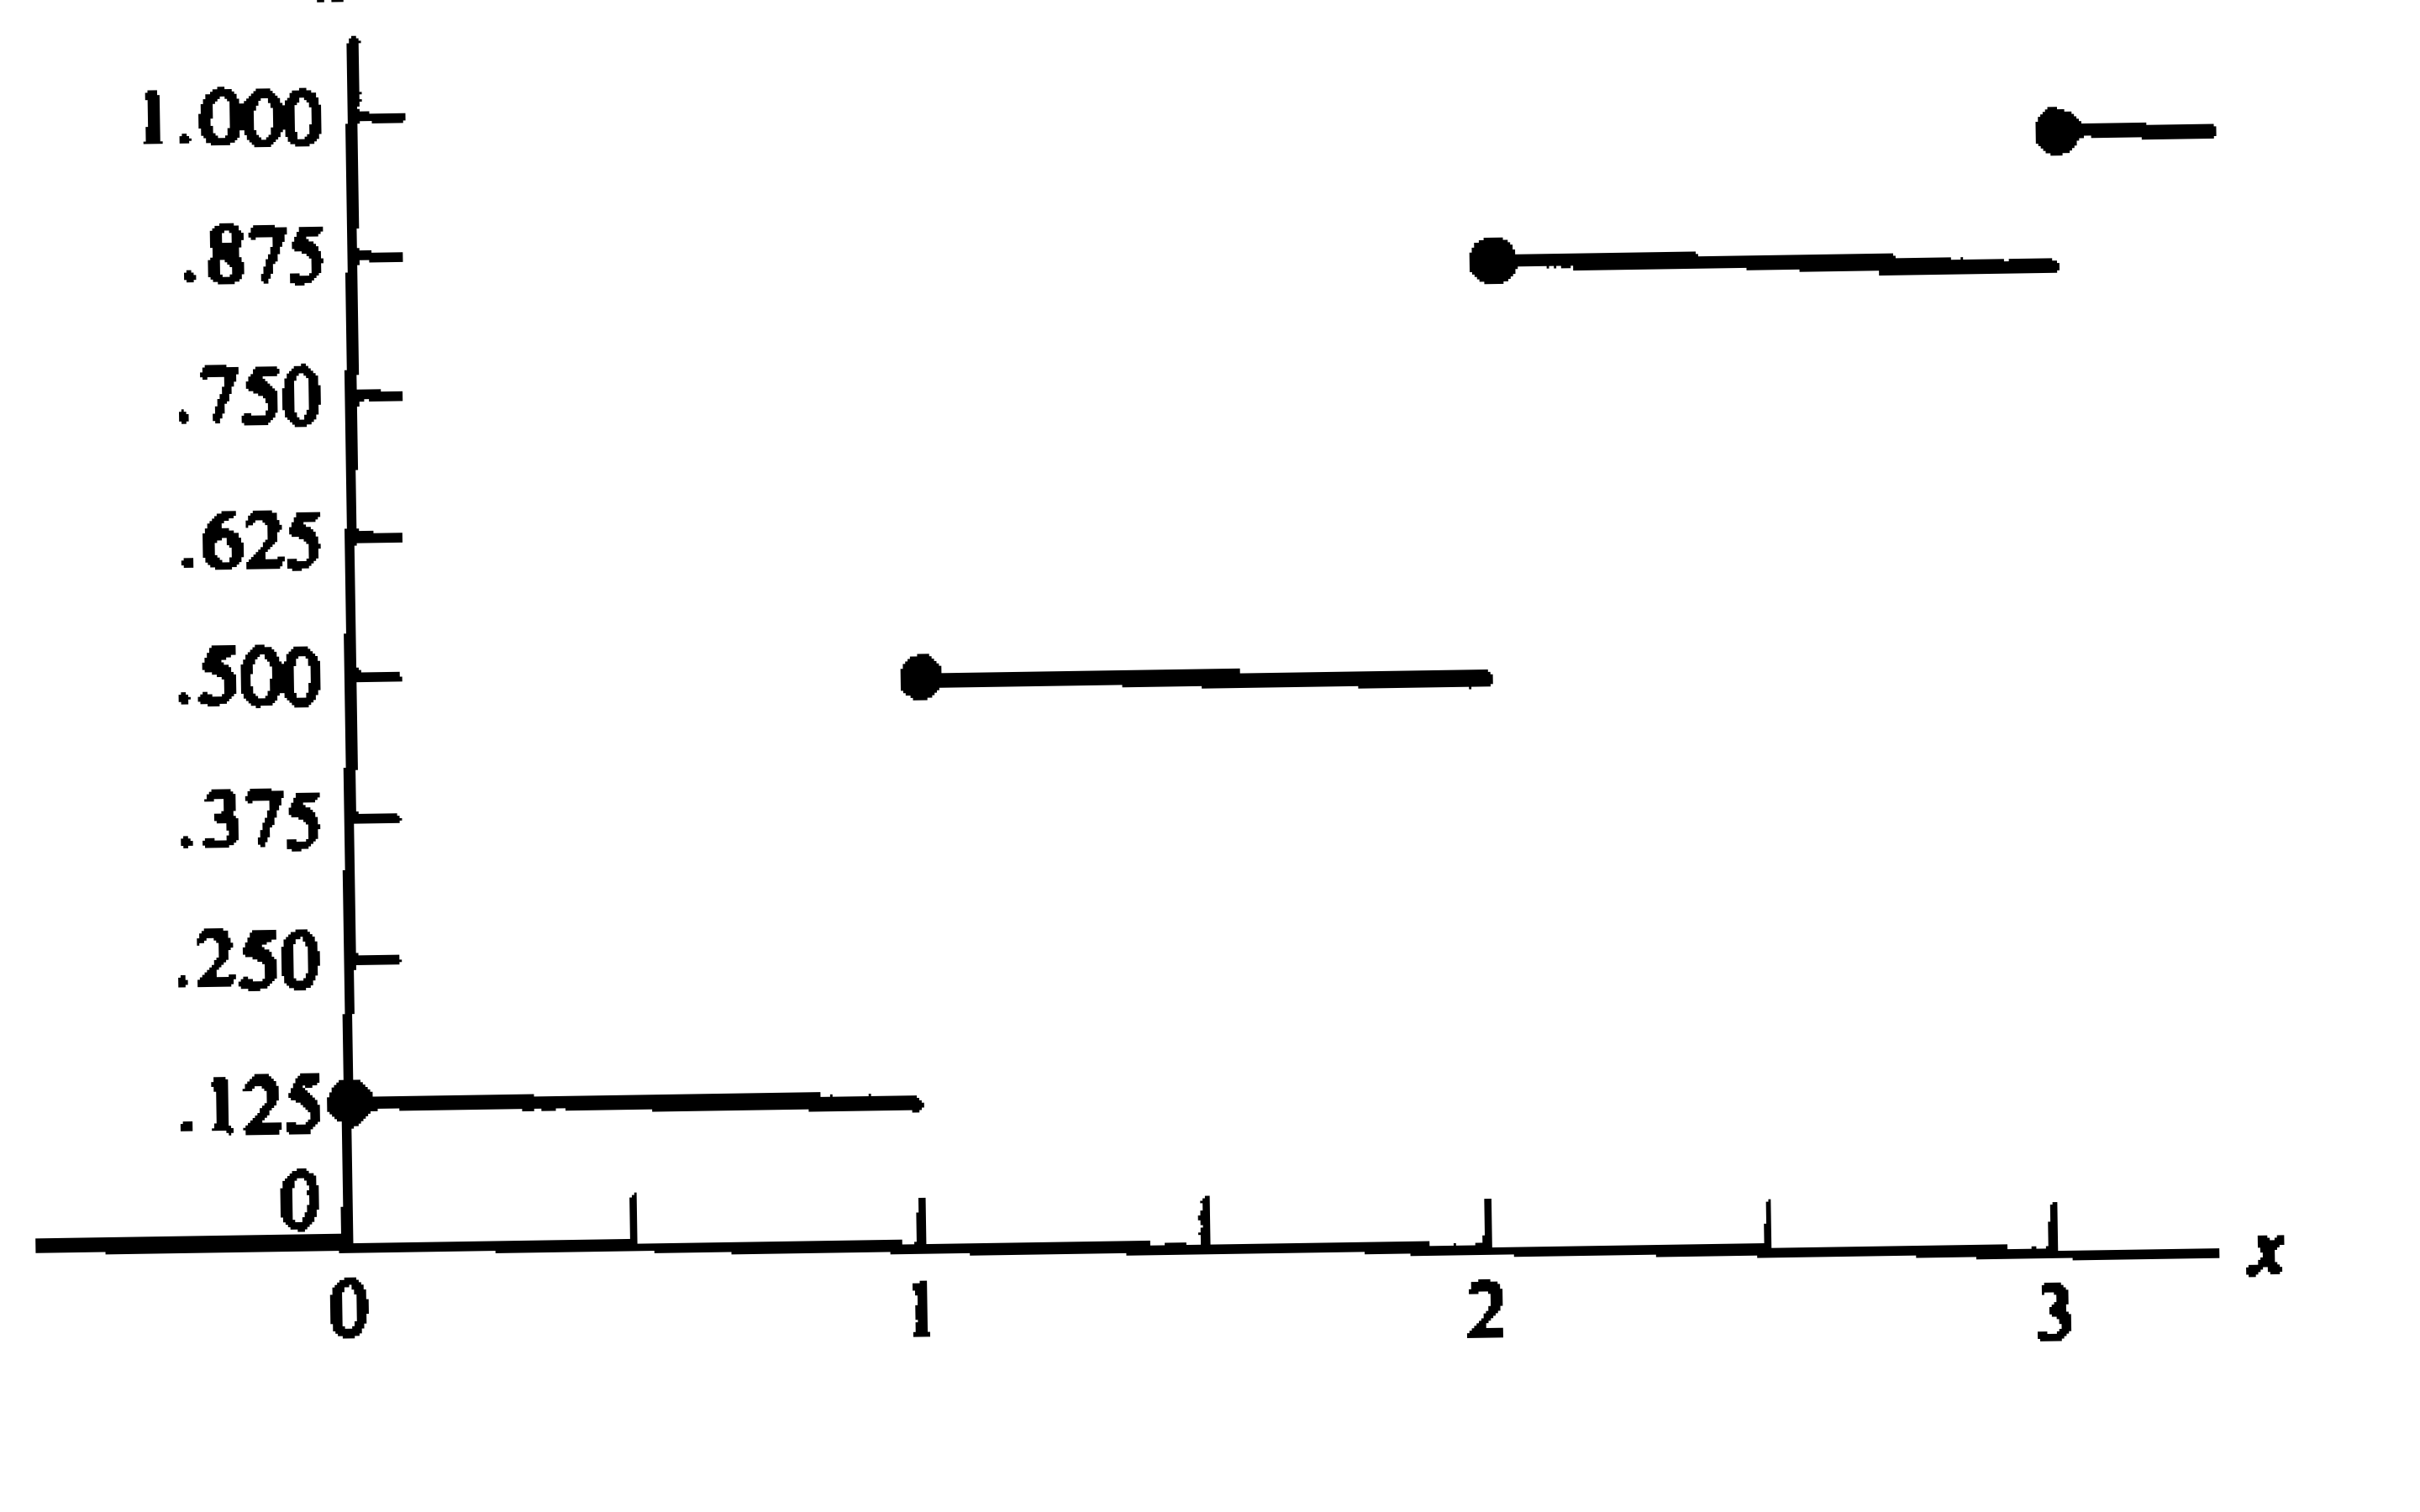
\includegraphics[scale=.13]{figs/CDF_three_coin_toss.png} 
\end{center}
\caption{ The polt of $F_X(x)$: CDF of the random variable X \vspace{-.15in}}
\end{figure}
\vspace{-.1in}
}
\qBox{
Note that $F_X(\cdot)$ is defined for all values of $x\in \R$, not just for $x\in \support{X}:=\{0,1,2,3\}$.  For example, $2.5 \notin \support{X}$,  however \vspace{-.18in}
$$ \HLTEQ[white]{F_X(2.5)= P_X(x\leq 2.5)= P_X(X=0)+P_X(X=1)+P_X(X=2)= \frac{7}{8}.}$$\vspace{-.25in}
}


\end{frame}




\TransitionFrame[airforceblue]{\Large Characterization of {\bf \it any} CDF Function}


\begin{frame}{Characterization of a CDF }

\begin{theorem}
The function $F(x)$ is a cdf { \bf   if and only if}  the following three conditions hold:
\begin{enumerate}
\item $\HLTW{\displaystyle \lim_{x\rightarrow -\infty } F(x)=0}$ and $\HLTW{\displaystyle \lim_{x\rightarrow \infty } F(x)=1}$. 
\item F(x) is a nondecreasing function of x
\item F(x) is right-continuous; that is, for every real  number $x_0$,  $\HLTY{\displaystyle \lim_{x\downarrow x_0} F(x)=  F(x_0)}$.
\end{enumerate}
\end{theorem}



\end{frame}


\begin{frame}

\qBox{
\HLTW{\text{Comment:}} Let $X$ be a random variable with the corresponding cdf $F_X(x)$ for $x\in \R$.  Let $x_0 \in \R$ is arbitrary. Then 
$$P(X=x_0):=P(X\in \{x_0\})=\HLTY{\displaystyle \lim_{\HLTW{x\downarrow x_0}} F_X(X)}-  \HLTY{\displaystyle\lim_{\HLTW{x\uparrow x_0}}F_X(x)}.$$
}
\end{frame}






\begin{frame}{Example: CDF continuous}
\begin{figure}
\begin{center}
\noindent\shadowimage[width=7cm]{figs/CDF_three_coin_toss.png}\par\bigskip 
\end{center}
\vspace{-.25in}
\caption{ The polt of $F_X(x)$: CDF of the random variable X}
\end{figure}

\vspace{-.1in}
\qBox{
Let $F_X(x)$ denotes the cdf function included in the above image. Therefore, \\
$\HLTEQ[yellow]{P(X=2)= \lim_{x\downarrow 2} F_X(X)-  \lim_{x\uparrow 2}F_X(x)= 0.5-0.125=0 .375.}$
$\HLTEQ[lightGreenOne]{P(X=1.5)= \lim_{x\downarrow 1.5} F_X(X)-  \lim_{x\uparrow 1.5}F_X(x)=0.5-0.5=0.}$
}


\end{frame}


\begin{frame}{Example: CDF continuous}
\qBox{{\bf Example:} An example of a continuous cdf is the function
$$ \displaystyle F_X(x):=\frac{1}{1+e^{-x}} \text{ for all } x\in \R.\vspace{-.2in}$$

\begin{figure}
\begin{center}
\noindent\shadowimage[width=6.3cm]{figs/logistic_CDF.png}\par\bigskip 
\end{center}
\vspace{-.25in}
\caption{ The polt of $F_X(x)$: CDF of the random variable X \vspace{-.1in}}
\end{figure}
}
Verify: The above function satisfies the three conditions required to be a  CDF.  
\end{frame}
 

\begin{frame}{Example:}

\qBox{\Qn: Prove that the following functions are valid cdfs. 
\begin{enumerate}
\item $F(x)= e^{	-e^{-x}}$ for all $x\in \R$. 
\item $F(x)= \frac{1}{2}+\frac{1}{\pi}\tan^{-1}(x)$ for all $x\in \R$. 	
\end{enumerate}


}

\vspace{1in}
\end{frame}




\begin{frame}
\define{Discrete Random Variable}{
A random variable X is discrete if it's support $\support[X]$ is finite or countable infinite. 
}


%\define{Alternative Definition: Discrete Random Variable}{
%A random variable X is discrete if the corresponding cdf $F_X(x)$ is a step function of x.  i.e.  $F_X(x)$ increases only via jumps. 
%}
\qBox{{\bf \HLTW{\text{ Alternative Characterization of Discrete Distributions: } }}
A random variable X is discrete if the corresponding cdf $F_X(x)$ is a step function of x.  i.e.  $F_X(x)$ increases only via jumps. 
}


\end{frame}






\section{Continuous Random Variables}
\TransitionFrame[airforceblue]{\Large Continuous Random Variables }

\begin{frame}{Continuous and Discrete Random variable}
\define{Continuous Random Variable}{
A random variable X is continuous if the corresponding cdf $F_x(x)$ is a continuous function of x. 
}

\end{frame}


\begin{frame}
\qBoxCol{lightBrownOne}{{\bf Question: }
Is it ture that a random variable must be continuous if its support is an interval ?
}\\

\qBoxCol{lightBrownOne}{{\bf Question: }
Is it ture that a random variable must be continuous if its support is $\R$?
}

\qBoxCol{lightBrownOne}{{\bf Question: }
Is it possible for a continuous random variable to have a finite support?
}
\end{frame}




\begin{frame}{Example: CDF continuous}
\qBox{{\bf Example:} An example of a continuous cdf is the function
$$ \displaystyle F_X(x):=\frac{1}{1+e^{-x}} \text{ for all } x\in \R.\vspace{-.2in}$$

\begin{figure}
\begin{center}
\noindent\shadowimage[width=6.3cm]{figs/logistic_CDF.png}\par\bigskip 
\end{center}
\vspace{-.25in}
\caption{ The polt of $F_X(x)$: CDF of the random variable X \vspace{-.1in}}
\end{figure}
}
Verify: The above function satisfies the three conditions required to be a  CDF.  
\end{frame}
 



\begin{frame}{Example: CDF continuous}
\qBox{{\bf Example of CDF of a Continuous Random Variable:} 
$$ F_X(x):= \left\{
\begin{array}{ll}
		0  & \mbox{if } x \leq  0 \\
		1- e^{-x}  & \mbox{if } x > 0
	\end{array}\right.
$$
}


{\bf Verify:} The above function satisfies the three conditions required to be a  CDF.
\end{frame}





\begin{frame}{Example:}

\qBox{\Qn: Prove that the following functions are valid cdfs. 
\begin{enumerate}
\item $F(x)= e^{	-e^{-x}}$ for all $x\in \R$. 
\item $F(x)= \frac{1}{2}+\frac{1}{\pi}\tan^{-1}(x)$ for all $x\in \R$. 	
\end{enumerate}


}

\end{frame}





\begin{frame}{Probability Density Function (pmf):  For  continuous  RV}

\define{Probability Density Function}{
The probability density function or pdf, $f_x(x)$, of a continuous random variable $X$ is the function that satisfies
$$F_X(x)= \int_{-\infty}^{x} f_x(x) dx $$\vspace{-.2in}
}

\qBox{{\bf Comment:}
Using the Fundamental Theorem of Calculus, if $f_X(x)$ is continuous, we have the further relationship  
$\displaystyle f_X(x)= \frac{d}{dx}F_{X}(x).$
 }
\qBox{
If X is a continuous random variable, then probabilities can be obtained by integrating its pdf over suitable region. Specifically, for $a, b\in \R$, $a<b$, 
$$\HLTEQ[white]{P(a< X\leq b)= F_X(b)-F_X(a)= \int_a^b f_{X}(x) dx.}$$\vspace{-.2in}
}

\end{frame}



\begin{frame}{Probability Density Function (pdf)}

\define{Continuous Random Variable}{
A random variable X is said to be continuous if there is a function $f(x)$, called the probability density function (pdf), such that
\begin{enumerate}
\item $f(x)\geq 0 $ for all $x$.
\item $\displaystyle \int_{-\infty}^{\infty}f(x)dx= 1$
\item $\HLTW{\displaystyle P(a\leq X\leq b)= \int_{a}^{b}f(x)dx}$ for all $a<b$.
\end{enumerate}
}

\qBrd[4.7in]{amethyst!40}{
\small
If $X$ is a continuous random variable then, 
\begin{itemize}
\item $P(X=c)= 0$ for any $c\in \R$
\item $P(a\leq X\leq  b) = P(a < X\leq b) = P(a\leq X < b) = P(a < X < b)$.
\end{itemize}
}

\end{frame}





\begin{frame}\frametitle{Example}

\vspace{-.1in}
\qbx[4.5in]{amethyst!40}{
\Exmpl{amethyst}{}  Suppose that $X$ is a continuous random variable whose probability density function is given by
$$ f(x):= \begin{cases} 
 C(4x-2x^2) & \text{ if } 0 <x<2\\
0 & \text{ otherwise.} 
\end{cases}$$
\vspace{-.1in}
\begin{enumerate}[a).]
\item What is the value of C?
\item Find $P(X>1)$.
\end{enumerate}
}\\
%\pause
\vspace{1.7in}
{\tiny {:}  
 
}
\end{frame}




\begin{frame}\frametitle{Example}
\tiny 
\vspace{-.1in}
\qbx[4.5in]{amethyst!40}{
\Exmpl{amethyst}{}  Suppose that $X$ is a continuous random variable whose probability density function is given by
$$ f(x):= \begin{cases} 
 C(4x-2x^2) & \text{ if } 0 <x<2\\
0 & \text{ otherwise.} 
\end{cases}$$
\vspace{-.1in}
\begin{enumerate}[a).]
\item What is the value of C?
\item Find $P(X>1)$.
\end{enumerate}
}\\

\begin{minipage}{.48\textwidth} %
{\tiny 
 \qBrd[1.6in]{babyblue!40}{
 According to the property of the pdf
 \begin{eqnarray}
& &  \int f(x)dx=1\nonumber\\
 & \implies&    \int_{0}^{2} C(4x-2x^2)dx=1\nonumber\\
 & \implies&     C(2x^2-\frac{2x^3}{3} )\Bigg\vert_{0}^2 =1\nonumber\\
  & \implies&     C(8-\frac{16}{3} ) =1\nonumber\\
   & \implies&     C =\frac{3}{8}\nonumber
 \end{eqnarray}
 }}
\end{minipage} %
\begin{minipage}{.48\textwidth} %
{\tiny 
 \qBrd[1.8in]{babyblue!40}{
 \begin{eqnarray}
 P(X>1)& = &   \int_{1}^{2} f(x)dx\nonumber\\
 & =&    \int_{1}^{2} C(4x-2x^2)dx\nonumber\\
 & =&     C(2x^2-\frac{2x^3}{3} )\Bigg\vert_{1}^2 =1\nonumber\\
  & =&     C\left\{ (8-\frac{16}{3} ) - (2-\frac{2}{3} )\right\} \nonumber\\
   & =&    C\left\{ \frac{8}{3} - \frac{4}{3} \right\}\nonumber\\
     & =&    \frac{3}{8}\times  \frac{4}{3}\nonumber\\
      & =&   \frac{1}{2}.\nonumber
 \end{eqnarray}
 }}
\end{minipage}

 
 
 

\end{frame}



\begin{frame}\frametitle{Example}

\vspace{-.1in}
\qbx[4.5in]{amber!40}{
\Exmpl{amber}{}  For a given IT technician in a support center, let X denote the percentage of time, out of a 40-hour work week, that he is directly serving customers. Suppose that X has a probability density function given by
$$ f(x):= \begin{cases} 
 3x^2& \text{ if } 0 <x<1\\
0 & \text{ otherwise.} 
\end{cases}$$
\vspace{-.1in}
\begin{enumerate}[a).]
\item Make a Graph of the above pdf. 
\item Find the probability that the technician will spend less than 30\% of his workweek serving customers.
\item Find the probability that the technician will spend 20\% to 70\% of hisworkweek serving customers.
\end{enumerate}
}\\
%\pause
\vspace{1.7in}
{\tiny {:}  
 
}
\end{frame}



\begin{frame}\frametitle{Example}
\tiny
\vspace{-.1in}
\qbx[4.5in]{amber!40}{
\Exmpl{amber}{}  For a given IT technician in a support center, let X denote the percentage of time, out of a 40-hour work week, that he is directly serving customers. Suppose that X has a probability density function given by
$$ f(x):= \begin{cases} 
 3x^2& \text{ if } 0 <x<1\\
0 & \text{ otherwise.} 
\end{cases}$$
\vspace{-.1in}
\begin{enumerate}[a).]
\item Make a Graph of the above pdf. 
\item Find the probability that the technician will spend less than 30\% of his workweek serving customers.
\item Find the probability that the technician will spend 20\% to 70\% of hisworkweek serving customers.
\end{enumerate}
}\\
%\pause

{\tiny 
\begin{minipage}{.29\textwidth} %
{\tiny 
 \qBrd[1.27in]{babyblue!40}{
 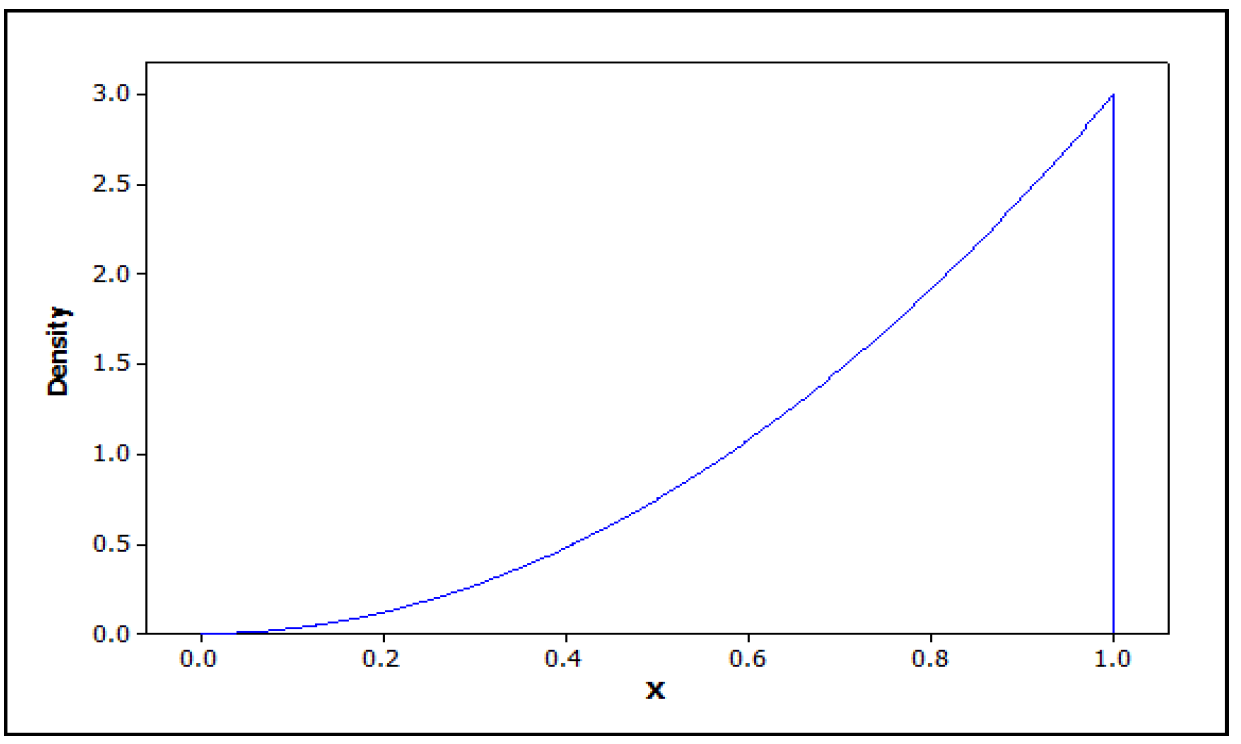
\includegraphics[scale=.15]{figs/pdf1.png}
 }}
\end{minipage} %
\begin{minipage}{.33\textwidth} %
{\tiny 
 \qBrd[1.4in]{babyblue!40}{
 \begin{eqnarray}
 P(X<0.3)& = &   \int_{0}^{0.3} f(x)dx\nonumber\\
 & =&    \int_{1}^{2} 3x^2dx\nonumber\\
 & =&     (x^3)\Bigg\vert_{0}^{0.3}\nonumber\\
     & =& (0.3)^3-(0)^3\nonumber\\
      & =&  0.027\nonumber
 \end{eqnarray}
 }}
\end{minipage}
\begin{minipage}{.31\textwidth} %
{\tiny 
 \qBrd[1.67in]{babyblueeyes!40}{
 \begin{eqnarray}
 P(0.2<X<0.7)& = &   \int_{0.2}^{0.7} f(x)dx\nonumber\\
 & =&    \int_{0.2}^{0.7} 3x^2dx\nonumber\\
 & =&    ( x^3)\Bigg\vert_{0.2}^{0.7}\nonumber\\
     & =& (0.7)^3-(0.2)^3\nonumber\\
      & =&0.337 \nonumber
 \end{eqnarray}
 }}
\end{minipage}

 
}
\end{frame}





\begin{frame}\frametitle{Exercise}

\vspace{-.1in}
\qbx[4.5in]{olive!40}{
\Exmpl{olive}{}  The amount of time in hours that a computer functions before
breaking down is a continuous random variable with probability
density function given by
$$ f(x):= \begin{cases} 
 100 e^{-\frac{x}{100}}& \text{ if } x> 0\\
0 & \text{ otherwise.} 
\end{cases}$$
What is the probability that
\vspace{-.1in}
\begin{enumerate}[a).]
\item a computer will function between 50 and 150 hours before breaking down?
\item it will function for fewer than 100 hours?
\end{enumerate}
}\\
%\pause
\vspace{1.7in}
{\tiny {:}  
 
}
\end{frame}




\begin{frame}\frametitle{Exercise}

\vspace{-.1in}
\qbx[4.5in]{applegreen!40}{
\Exmpl{applegreen}{}  The lifetime in hours of a certain kind of radio tube is a random
variable having a probability density function given by
$$ f(x):= \begin{cases} 
\frac{100}{x^2}& \text{ if } x> 100\\
0 & \text{if 	$ x\leq 100$.} 
\end{cases}$$
What is the probability that exactly 2 of 5 such tubes in a radio set
will have to be replaced within the  fist 150 hours of operation?
{\tiny Assume that the events $E_i$, $i = 1,2,3,4,5, $that the ith such tube will have to be replaced within this time are independent.}
}\\
%\pause
\vspace{1.7in}
{\tiny {:}  
 
}
\end{frame}



\begin{frame}{Cumulative Distribution Function (cdf)}
\define{(The Cumulative Distribution Function)}{
The cumulative distribution function (cdf) F(x) of a continuous random variable $X$ with pdf $f()$ is defined for every number $x$ by $$ F(x)=P(X\leq x)= \int_{-\infty}^{x}f(x) dx.$$
}

\qBrd[4.5in]{amethyst!40}{
\qBrd[1.7in]{amethyst!70}{A Few Properties of F(x)}
\begin{enumerate}
\item $P(a< X\leq  b) = F(b) - F(a).$
\item  $P(X>  b) = 1-F(b)$
\item If X is a continuous random variable with cdf $F(x)$ then at every x at which $\frac{dF(x)}{dx}$ exists:
$f(x)=\frac{dF(x)}{dx} $
\end{enumerate}
}
\end{frame}


\begin{frame}\frametitle{Example}

\vspace{-.1in}
\qbx[4.5in]{apricot!50}{
\Exmpl{apricot}{}  For a given IT technician in a support center, let X denote the percentage of time, out of a 40-hour work week, that he is directly serving customers. Suppose that X has a probability density function given by
$$ f(x):= \begin{cases} 
{3x^2}& \text{ if }0\leq  x\leq 1\\
0 & \text{therwise.} 
\end{cases}$$
\vspace{-.1in}
\begin{enumerate}[a).]
\item Obtain, $F(x)$, the CDF of X.
\item Use $F(x)$ to compute  $P(0.5<X\leq 0.8)$.
\end{enumerate}
}
{\tiny {:}  
 
}
\end{frame}




\begin{frame}\frametitle{Example}
\tiny
\vspace{-.1in}
\qbx[4.5in]{apricot!40}{
\Exmpl{apricot}{}  For a given IT technician in a support center, let X denote the percentage of time, out of a 40-hour work week, that he is directly serving customers. Suppose that X has a probability density function given by
$$ f(x):= \begin{cases} 
 3x^2& \text{ if } 0 <x<1\\
0 & \text{ otherwise.} 
\end{cases}$$
\vspace{-.1in}
\begin{enumerate}[a).]
\item Obtain, $F(x)$, the CDF of X and Graph it.
\item Use $F(x)$ to compute  $P(0.5<X\leq 0.8)$.
\end{enumerate}
}\\
%\pause
{\tiny 
\begin{minipage}{.33\textwidth} %
{\tiny 
 \qBrd[1.6in]{babyblue!40}{
 \begin{eqnarray}
 F(x)= P(X\leq x)& =&    \int_{0}^{x} f(y)dy\nonumber\\
 & =&    \int_{0}^{x} 3y^2dy\nonumber\\
 & =&     (y^3)\Bigg\vert_{0}^{x}\nonumber\\
     & =& x^3\nonumber
 \end{eqnarray}
 $$\HLTW{ F(x)= \begin{cases}
 0 & \text{ if } x<0\\
 x^2 & \text{ if } 0 \geq x<1\\
 1 & \text{ if } x\geq 1.\\
 \end{cases}  }$$
 }}
\end{minipage}
\hspace{.1in}
\begin{minipage}{.29\textwidth} %
{\tiny 
 \qBrd[1.4in]{babyblue!40}{
 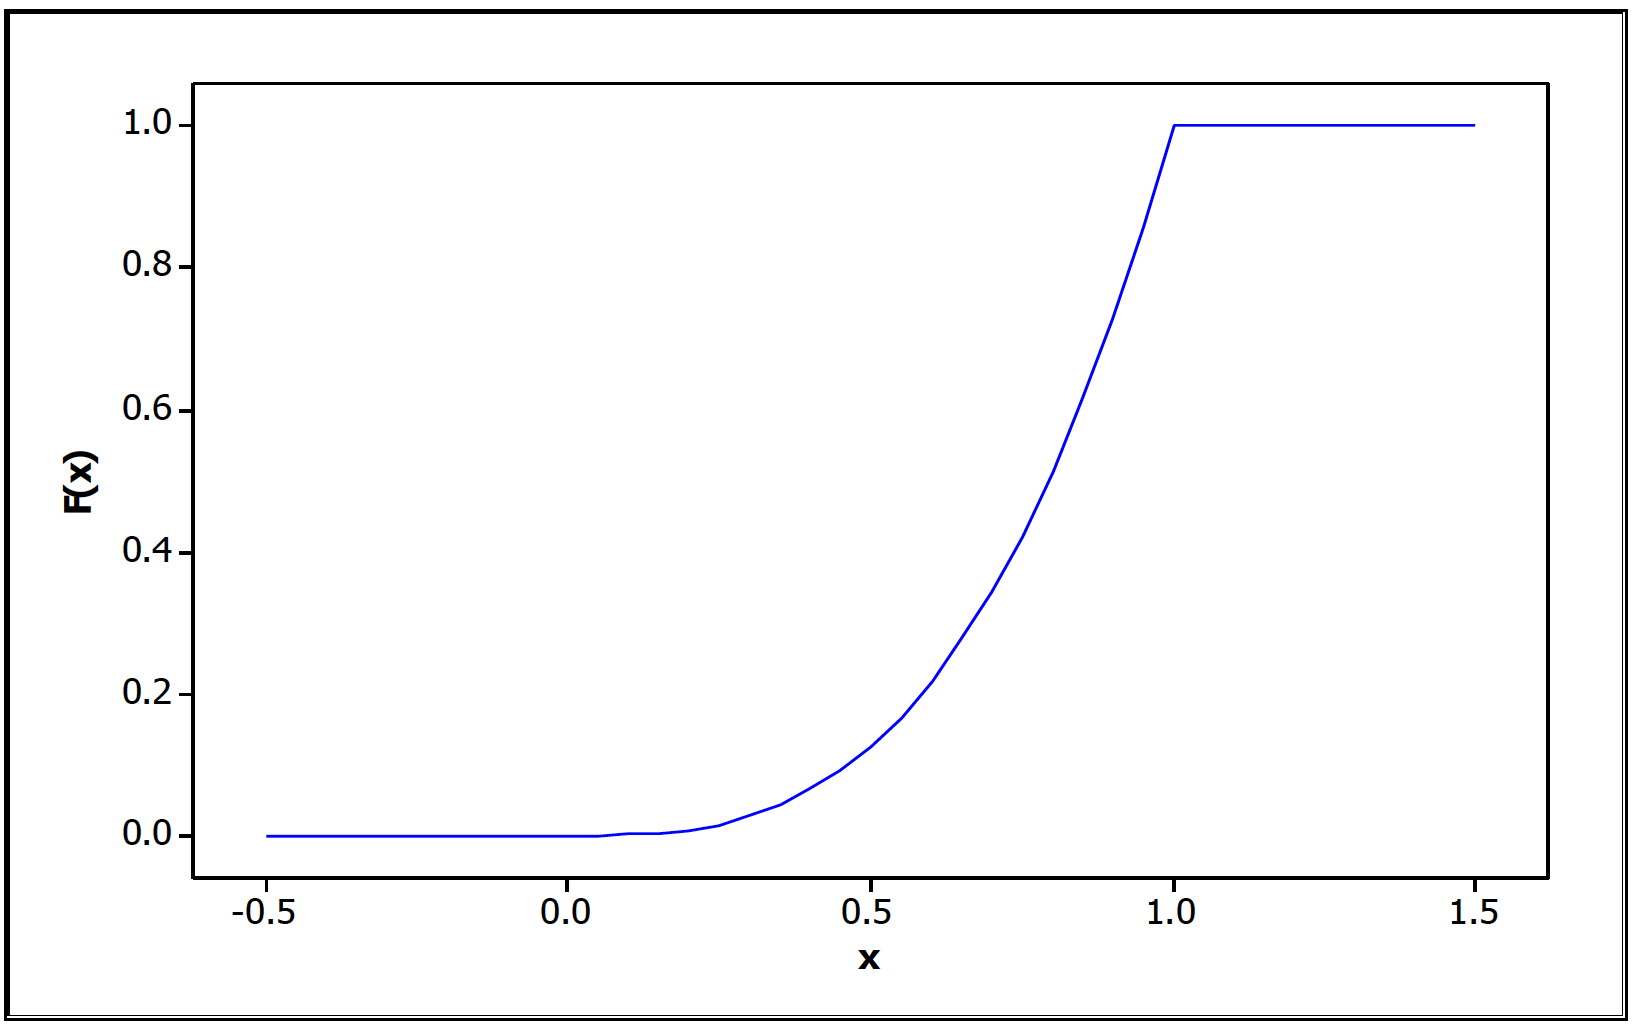
\includegraphics[scale=.12]{figs/CDF1.png}
 }}
\end{minipage} %
\hspace{.1in}
\begin{minipage}{.31\textwidth} %
{\tiny 
 \qBrd[1.45in]{babyblueeyes!40}{
 \begin{eqnarray}
& &  P(0.5<X<0.8)\nonumber\\
 & = &  F(0.8)- F(0.5)\nonumber\\
 &  =& ( 0.8)^3-(0.5)^3\nonumber\\
 & =&  0.387\nonumber
 \end{eqnarray}
 }}
\end{minipage}

 
}
\end{frame}






\begin{frame}\frametitle{Example}

\vspace{-.1in}
\qbx[4.5in]{teal!40}{
\Exmpl{teal}{} Let X be a continuous random variable  with Cumulative Distribution Function F(x),  and density function f(x). 
\begin{enumerate}
\item Obtain the cumulative  distribution function of $Y = 2X$.
\item Obtain the probability density function of $Y = 2X$.
\end{enumerate}
}
{\tiny {:}  
 
}
\vspace{3in}
\end{frame}




\begin{frame}\frametitle{Percentiles, Quantiles, and Median}
\vspace{-.1in}
\define{Percentiles}{
Let $p$ be a number between 0 and 1. The $(100)^{\text{th}}$ percentile of the distribution of a continuous random variable X, we shall denote by c, is that value for which
$$ F(c)= p$$
i.e. $c= F^{-1}(p)$.
where $F^{-1}(\cdot)$ is the inverse cumulative distribution function.
}

\qBrd{babyblue!50}{
Special percentiles:
\begin{enumerate}
\item The median of a continuous distribution, denoted by m, is the 50th percentile. So $m$ satisfies  $m = F^{-1}(0.5)$.
\item The first and the third quartiles can be computed as $Q_1=  F^{-1}(0.25)$
\item The third and the third quartiles can be computed as $Q_3=  F^{-1}(0.75)$
\end{enumerate}
}

\vspace{.2in}
\end{frame}






\begin{frame}\frametitle{Example}
\vspace{-.1in}
\qbx[4.5in]{apricot!40}{
\Exmpl{apricot}{}  For a given IT technician in a support center, let X denote the percentage of time, out of a 40-hour work week, that he is directly serving customers. Suppose that X has a probability density function given by
$$ f(x):= \begin{cases} 
 3x^2& \text{ if } 0 <x<1\\
0 & \text{ otherwise.} 
\end{cases}$$
\vspace{-.1in}
\begin{enumerate}[a).]
\item find the median, and 
\item the interquartile range of the distribution.
\end{enumerate}
}\\
%\pause

\end{frame}





\begin{frame}\frametitle{Example}
\tiny
\vspace{-.1in}
\qbx[4.5in]{apricot!40}{
\Exmpl{apricot}{}  For a given IT technician in a support center, let X denote the percentage of time, out of a 40-hour work week, that he is directly serving customers. Suppose that X has a probability density function given by
$$ f(x):= \begin{cases} 
 3x^2& \text{ if } 0 <x<1\\
0 & \text{ otherwise.} 
\end{cases}$$
\vspace{-.1in}
\begin{enumerate}[a).]
\item find the median, and 
\item the interquartile range of the distribution.
\end{enumerate}
}\\
%\pause
{\tiny 
\begin{minipage}{.33\textwidth} %
{\tiny 
 \qBrd[1.6in]{babyblue!40}{
 We have already Shown
 $$\HLTW{ F(x)= \begin{cases}
 0 & \text{ if } x<0\\
 x^2 & \text{ if } 0 \geq x<1\\
 1 & \text{ if } x\geq 1.\\
 \end{cases}  }$$
 Note that if $F(x)= y\implies x^3=y \implies x= y^{\frac{1}{3}} \implies F^{-1}(y)= y^{\frac{1}{3}}.$
 }}
\end{minipage}
\hspace{.1in}
\begin{minipage}{.29\textwidth} %
{\tiny 
 \qBrd[1.4in]{babyblue!40}{
 $m= F^{-1}(0.5)= (0.5)^{\frac{1}{3}}= 0.794$
 }}
\end{minipage} %
\hspace{.1in}
\begin{minipage}{.31\textwidth} %
{\tiny 
 \qBrd[1.45in]{babyblueeyes!40}{
 \begin{eqnarray}
&&  \text{IQR} \nonumber\\
& =&  Q_3-Q_1 \nonumber\\
 & =& F^{-1}(0.75) - F^{-1}(0.25)\nonumber\\
 & =&  (0.75)^{\frac{1}{3}}- (0.25)^{\frac{1}{3}}\nonumber\\
  & =  & 0.909 -0.630\nonumber\\
   &  =&  0.279\nonumber
 \end{eqnarray}
 }}
\end{minipage}

 
}
\end{frame}




\section{Expected Value, Variance \& MGF of a Continuous Random Variable }

\TransitionFrame[airforceblue]{\Large Expected Value,  Variance , \& MGF of a Continuous Random Variable }




\begin{frame}{Expected Value, or   {\bf mean } of a Continuous Random Variable}
\define{Expected Value or {\bf mean } of a Continupues Random Variable}{
If X is a continuous random variable with pdf $f(x)$, then the expected value (the mean) of X denoted by $E(X)$ or $ \mu_{_X}$ is given by
$$\mu_{_X}:= E(X)= \int_{-\infty}^{\infty} xf(x)dx$$
}
\end{frame}




\begin{frame}{}
\define{Expected Value of a function of a Continuous Random Variable}{
Let h(x) be any$^{*}$ function.  If X is a continuous random variable with pdf $f(x)$, then the expected value $h(X)$ denoted by $E(h(X))$ is given by
$$ E(h(X))= \int_{-\infty}^{\infty} h(x)f(x)dx$$
}
\end{frame}




\begin{frame}{Variance of a  Random Variable}
\define{Variance a Random Variable}{
Variance of a random variable $X$ is defined to be 
$$ \text{Var}(X)= E(X^2)- \left( E(X) \right)^2$$
}
\end{frame}


\begin{frame}\frametitle{A Few Properties of Expected Value and Variance of a Random Variable}
\qBrd{teal!40}{
Let $a$ and $b$ are constants, then 
\begin{enumerate}
\item $E(a+bX)= a+bE(X)$
\item $\text{Var}(a+bX)=b^2\text{Var}(X)$
\end{enumerate}
}

\end{frame}




\section{A Few Examples }

\TransitionFrame{A Few Examples }


\begin{frame}\frametitle{Example}
\vspace{-.1in}
\qbx[4.5in]{apricot!40}{
\Exmpl{apricot}{}  For a given IT technician in a support center, let X denote the percentage of time, out of a 40-hour work week, that he is directly serving customers. Suppose that X has a probability density function given by
$$ f(x):= \begin{cases} 
 3x^2& \text{ if } 0 <x<1\\
0 & \text{ otherwise.} 
\end{cases}$$
\vspace{-.1in}
\begin{enumerate}[a).]
\item Find the expected value of percentage of time the technician spends serving customers.
\item variance of percentage of time the technician spends serving customers.
\end{enumerate}
}\\

\end{frame}





\begin{frame}\frametitle{Example}
\tiny
\vspace{-.1in}
\qbx[4.5in]{apricot!40}{
\Exmpl{apricot}{}  For a given IT technician in a support center, let X denote the percentage of time, out of a 40-hour work week, that he is directly serving customers. Suppose that X has a probability density function given by
$$ f(x):= \begin{cases} 
 3x^2& \text{ if } 0 <x<1\\
0 & \text{ otherwise.} 
\end{cases}$$
\vspace{-.1in}
\begin{enumerate}[a).]
\item Find the expected value of percentage of time the technician spends serving customers.
\item variance of percentage of time the technician spends serving customers.
\end{enumerate}
}\\
%\pause
{\tiny 
\begin{minipage}{.33\textwidth} %
{\tiny 
 \qBrd[1.6in]{babyblue!40}{
\begin{eqnarray*}
E(X)
& =& \int_{-\infty}^{\infty}x f(x) dx\\
& =& \int_{0}^{1}x (3x^2) dx\\
& =& \int_{0}^{1} (3x^3) dx\\
& =& \frac{3x^4}{4} \Big\vert _{0}^{1}\\
& =& \frac{3}{4}\\
\end{eqnarray*}
 }}
\end{minipage}
\hspace{.1in}
\begin{minipage}{.29\textwidth} %
{\tiny 
 \qBrd[1.4in]{babyblue!40}{
 \begin{eqnarray*}
E(X^2)
& =& \int_{-\infty}^{\infty}x^2 f(x) dx\\
& =& \int_{0}^{1}x^2 (3x^2) dx\\
& =& \int_{0}^{1} (3x^4) dx\\
& =& \frac{3x^5}{5} \Big\vert _{0}^{1}\\
& =& \frac{3}{5}\\
\end{eqnarray*}
 }}
\end{minipage} %
\hspace{.1in}
\begin{minipage}{.31\textwidth} %
{\tiny 
 \qBrd[1.45in]{babyblueeyes!40}{
 \begin{eqnarray*}
&&  \text{Var}(X) \nonumber\\
& =&  E(X^2)- \left(E(X)\right)^2 \nonumber\\
   &  =&   \frac{3}{5}- \left( \frac{3}{4}\right)^2\\
    &  =&   0.6- \left( 0.75\right)^2\\
    & =& 0.0375
 \end{eqnarray*}
 }}
\end{minipage}

 
}
\end{frame}













\begin{frame}\frametitle{Example}
\vspace{-.1in}
\qbx[4.5in]{amethyst!40}{
\Exmpl{amethyst}{}  Find $E(X)$ and Var$(X)$ when the density function of X is
$$ f(x):= \begin{cases} 
 2x& \text{ if } 0 \leq x\leq 1\\
0 & \text{ otherwise.} 
\end{cases}$$
}\\
%\pause


\end{frame}





\begin{frame}\frametitle{Example}
\tiny
\vspace{-.1in}
\qbx[4.5in]{amethyst!40}{
\Exmpl{amethyst}{}  Find $E(X)$ and Var$(X)$ when the density function of X is
$$ f(x):= \begin{cases} 
 2x& \text{ if } 0 \leq x\leq 1\\
0 & \text{ otherwise.} 
\end{cases}$$
}\\
%\pause
{\tiny 
\begin{minipage}{.33\textwidth} %
{\tiny 
 \qBrd[1.6in]{babyblue!40}{
\begin{eqnarray*}
E(X)
& =& \int_{-\infty}^{\infty}x f(x) dx\\
& =& \int_{0}^{1}x (2x) dx\\
& =& \int_{0}^{1} (2x^2) dx\\
& =& \frac{2x^3}{3} \Big\vert _{0}^{1}\\
& =& \frac{2}{3}\\
\end{eqnarray*}
 }}
\end{minipage}
\hspace{.1in}
\begin{minipage}{.29\textwidth} %
{\tiny 
 \qBrd[1.4in]{babyblue!40}{
 \begin{eqnarray*}
E(X^2)
& =& \int_{-\infty}^{\infty}x^2 f(x) dx\\
& =& \int_{0}^{1}x^2 (2x) dx\\
& =& \int_{0}^{1} (2x^3) dx\\
& =& \frac{2x^4}{4} \Big\vert _{0}^{1}\\
& =& \frac{2}{4}\\
& =& \frac{1}{2}
\end{eqnarray*}
 }}
\end{minipage} %
\hspace{.1in}
\begin{minipage}{.31\textwidth} %
{\tiny 
 \qBrd[1.45in]{babyblueeyes!40}{
 \begin{eqnarray*}
&&  \text{Var}(X) \nonumber\\
& =&  E(X^2)- \left(E(X)\right)^2 \nonumber\\
   &  =&   \frac{1}{2}- \left( \frac{2}{3}\right)^2\\
    &  =&    \frac{1}{2}-  \frac{4}{9}\\
    & =&  \frac{10}{9}
 \end{eqnarray*}
 }}
\end{minipage}

 
}
\end{frame}







\begin{frame}\frametitle{Example}
\vspace{-.1in}

\qbx[4.5in]{applegreen!40}{
\Exmpl{applegreen}{}  Find $E(e^X)$ when the density function of X is
$$ f(x):= \begin{cases} 
 1& \text{ if } 0 \leq x\leq 1\\
0 & \text{ otherwise.} 
\end{cases}$$
}\\
\vspace{2in}


\end{frame}

\begin{frame}\frametitle{Example}
\vspace{-.1in}

\qbx[4.5in]{applegreen!40}{
\Exmpl{applegreen}{}  Find $E(e^X)$ when the density function of X is
$$ f(x):= \begin{cases} 
 1& \text{ if } 0 \leq x\leq 1\\
0 & \text{ otherwise.} 
\end{cases}$$
}\\
%\pause
{\tiny 
 \qBrd[4.4in]{olive!40}{
 \begin{eqnarray*}
E(e^X)
& =& \int_{-\infty}^{\infty}e^x f(x) dx\\
& =& \int_{0}^{1}e^x (1) dx\\
& =&e^x \Big\vert _{0}^{1}\\
& =&e^1-e^0\\
& =& e-1
\end{eqnarray*}
 }}


\end{frame}









\begin{frame}\frametitle{Exercise}
\tiny
\vspace{-.1in}
\qbx[4.5in]{amethyst!40}{
\Exmpl{amethyst}{}  Let X denote the resistance of a randomly chosen resistor, and suppose that its pdf is given by
$$ f(x):= \begin{cases} 
 \frac{x}{18}& \text{ if } 8 \leq x\leq 10\\
0 & \text{ otherwise.} 
\end{cases}$$
\begin{enumerate}
\item Find and graph the cdf of X.
\item  Find $P(8.6< X\leq 9:8)$.
\item Find the median of the resistance of such resistors.
\item Find the mean and variance of X.
\end{enumerate}
}\\
%\pause
\vspace{1.5in}
\end{frame}



\begin{frame}\frametitle{Exercise}
\tiny
\vspace{-.1in}
\qbx[4.5in]{bittersweet!40}{
\Exmpl{bittersweet}{}  The length of time to failure (in hundreds of hours) for a transistor is a random variable X with cumulative distribution function given by
$$ F(x):= \begin{cases} 
1- e^{-x^2}& \text{ for }x>0\\
0 & \text{ otherwise.} 
\end{cases}$$
\begin{enumerate}
\item Find a pdf of X $f(x)$. 
\item  Find the probability that the transistor operates for at least 200 hours.
\item Find the $30^{\text{th}} $ percentile of X.
\end{enumerate}
}\\
%\pause
\vspace{1.5in}
\end{frame}






\begin{frame}\frametitle{Exercise}
\tiny
\vspace{-.1in}
\qbx[4.5in]{bluebell!40}{
\Exmpl{bluebell}{}  Weekly CPU time used by an accounting firm has probability density function (measured in hours) given by
$$ f(x):= \begin{cases} 
\frac{3}{64}x^2(4-X)& \text{ for }0\leq x\leq 4\\
0 & \text{ otherwise.} 
\end{cases}$$
\begin{enumerate}
\item Find the F(x) for weekly CPU time.
\item  Find the probability that the of weekly CPU time will exceed two hours for a selected week.
\item Find the expected value and variance of weekly CPU time.
\item Find the probability that the of weekly CPU time will be within half an hour of the expected weekly CPU time.
\item The CPU time costs the firm \$200 per hour. Find the expected value and variance of the weekly cost for CPU time.
\end{enumerate}
}\\
%\pause
\vspace{1.5in}
\end{frame}





\begin{frame}\frametitle{Exercise}
\tiny
\vspace{-.1in}
\qbx[4.5in]{asparagus!40}{
\Exmpl{asparagus}{}  The length of time required by students to complete a one-hour exam is a random variable with a density function given by
$$ f(x):= \begin{cases} 
cy^2+y& \text{ for }0\leq x\leq 1\\
0 & \text{ otherwise.} 
\end{cases}$$
\begin{enumerate}
\item Find c that makes this function a valid probability density function.
\item Find the F(y) 
\item Graph f(y) and F(y).
\item  Find the probability that a randomly selected student will finish in less than half an hour.
\item Find the time that 95\% of the students finish before it.
\item Given that a particular student needs at least 15 minutes to complete the exam, find the probability that she will require at least 30 minutes to finish.
\end{enumerate}
}\\
%\pause
\vspace{1.5in}
\end{frame}







%\section{Moment Generating Function}
%\TransitionFrame[airforceblue]{\Large Simulations  }

%
%\section{Moment Generating Function}
%\TransitionFrame[airforceblue]{\Large Moment Generating Function  }

%\TransitionFrame[airforceblue]{\Large  A }





\TransitionFrame[antiquefuchsia]{\Large Questions?  }
 
 
\end{document}
